%% Elastic Perimeter Disk Model — Physical Review E two-column format
%% Compile: xelatex main.tex  (run twice for cross-references)
\documentclass[aps,pre,twocolumn,floatfix,longbibliography]{revtex4-2}

\usepackage{amsmath,amssymb}
\usepackage{graphicx}
\usepackage{booktabs}
\usepackage{xcolor}
\usepackage{hyperref}
\usepackage{microtype}
\usepackage{listings}
\lstset{basicstyle=\ttfamily\footnotesize, breaklines=true,
        frame=single, backgroundcolor=\color{gray!8}}

% Convenience macros
\newcommand{\El}{E_l}
\newcommand{\Elb}{E_l^{\mathrm{base}}}
\newcommand{\Elc}{E_l^{\mathrm{code}}}
\newcommand{\Karea}{K_{\mathrm{area}}}
\newcommand{\numes}{\nu_{\mathrm{meas}}}
\newcommand{\dA}{\Delta A}
\newcommand{\eref}{\varepsilon_{\mathrm{ref}}}
\newcommand{\ep}{\varepsilon_p}
\newcommand{\SR}{\mathrm{SR}}
\newcommand{\cv}{\mathrm{CV}}

\begin{document}

\title{The Elastic Perimeter Disk Model:\\
       Construction, Parameterization, and Calibration}

\author{Research Note}
\date{\today}

\begin{abstract}
We construct and calibrate the \emph{Elastic Perimeter Disk} (EPD) model, a minimal
2D particle model in which a single dimensionless parameter $q$ continuously tunes
particle squishiness from nearly area-compressible ($\nu \approx 0.17$) to nearly
incompressible ($\nu \approx 0.94$).  Each disk is represented by $N$ perimeter
nodes; the elastic energy comprises membrane stretching, bending, and a soft area
penalty.  Dimensional analysis reduces the full parameter space to two physically
interpretable dimensionless numbers: the bending number $b = \tau^2/12$ and the area
stiffness ratio $q = \Karea/\Elb$.  Fixing $b = 0.2$ and sweeping $q$ over three
decades traces a clean, monotone squishiness axis in the two-disk flat-wall squeeze
geometry.  A calibration sweep extended to $N \in \{32, 48, 72, 120, 240\}$ reveals a
systematic $N$-dependence: $\Delta\nu < 0.01$ within the $N \leq 72$ band but
$\Delta\nu \leq 0.046$ across the full range, necessitating resolution-matched
recalibration at the production tier $N = 240$.  A spot-check at $R_0 \in \{0.5, 1.0, 2.0\}$
confirms exact $R_0$-invariance ($\cv < 0.01\%$) to floating-point precision.  The
resulting recipe maps any target Poisson ratio $\nu_{\rm target} \in (0.17, 0.94)$
and particle radius $R_0$ to a unique, validated parameter set.  The disk-disk
contact force obeys $F_{\rm dd} \propto \delta^n$ with $n(N) = n_\infty + a/N$
($a \approx 16$--$17$, $n_\infty \approx 0.92$--$0.97$); at $N = 240$ the measured
exponent is $n \approx 1.00$--$1.09$ (slightly super-linear to nearly linear), while $N = 32$ yields
$n \approx 1.5$ (a resolution artefact mimicking 3D Hertz).  We additionally
present a rigid-body decomposition integrator that is verified to machine precision
via 48-case direct impulse tests, extend the model to non-circular
\texttt{EllipseParticle} shapes (angular momentum conserved to $< 10^{-12}$ in four
collision configurations), and derive a bending-mode theory for the damping parameter
that quantifies the COR--ringing tradeoff: $\text{COR}$ varies from 0.89 to 0.26
as $\alpha_d$ is swept from $Q = 20$ to $Q = 0.3$.
Supplemental movies (Movies~S1--S8) illustrate the full squishiness axis and
multi-body collision dynamics.
\end{abstract}

\maketitle

%%============================================================
\section{Motivation and Scope}
\label{sec:motivation}
%%============================================================

A central question in the mechanics of dense soft-particle systems is how particle
\emph{squishiness}---the ease with which a particle deforms under contact---governs
collective behavior near the jamming point~\cite{OHern2003,vanHecke2010}.  In
continuum solid mechanics, the Poisson ratio $\nu$ parameterizes this axis cleanly:
$\nu = 0$ corresponds to a fully compressible material, while $\nu \to 1/2$ in 2D
corresponds to an incompressible material that conserves area at the cost of lateral
deformation.  A granular analog of $\nu$---a single dimensionless knob spanning the
full range from area-compressible to shape-deformable particles---would allow
systematic exploration of jamming mechanics without committing to a specific material
model.

Full FEM-DEM simulations~\cite{Li2020IPC,Treado2021} provide this control in
principle, but are computationally prohibitive for large assemblies
($N_p \gtrsim 100$ particles), require detailed constitutive laws, and expose many
parameters whose effects on collective dynamics are not individually transparent.

We instead construct the \textbf{Elastic Perimeter Disk (EPD)} model, whose only
representation of the particle interior is through forces on a discretized perimeter.
The model is designed around a single question: what is the minimum set of elastic
energy terms on the perimeter that produces a tunable, Poisson-ratio-like knob?  We
show that three terms suffice---membrane stretching, bending, and an area
penalty---and that the model's behavior reduces through dimensional analysis to two
physically interpretable dimensionless parameters.  One combination is fixed as a
working point, and the remaining parameter $q$ controls a smooth squishiness axis from
$\nu \approx 0.17$ to $\nu \approx 0.94$.  The calibration curve $q \mapsto \nu$
allows a user to specify $\nu_{\rm target}$ and have all simulation parameters
determined uniquely (Sec.~\ref{sec:recipe}).

%%============================================================
\section{Geometry and Degrees of Freedom}
\label{sec:geometry}
%%============================================================

\subsection{Particle discretization}

Each particle is a 2D disk of reference radius $R_0$.  The perimeter is discretized
as $N$ nodes on the reference circle:
\begin{equation}
  \mathbf{X}_i = R_0 \bigl(\cos(2\pi i/N),\, \sin(2\pi i/N)\bigr),
  \quad i = 0,\ldots,N-1,
\label{eq:ref_config}
\end{equation}
with reference edge length $L_0 = 2\pi R_0/N$ and reference curvature
$\kappa_0 = 1/R_0$.  At time $t$, node $i$ occupies position $\mathbf{x}_i(t)$;
the elastic displacement is $\mathbf{u}_i = \mathbf{x}_i - \mathbf{X}_i$.  No
small-deformation assumption is made: all geometric quantities are evaluated
exactly from $\{\mathbf{x}_i\}$ at each timestep.

\subsection{Contact radius and effective size}

Each perimeter edge is treated as a line segment of half-width $r_c = L_0$, giving
the particle a capsule geometry.  The effective particle radius is
$R_{\rm eff} = R_0(1 + 2\pi/N)$.  In multi-particle simulations, packing fractions
must be computed using $R_{\rm eff}$, not $R_0$.

%%============================================================
\section{Elastic Energy Functional}
\label{sec:energy}
%%============================================================

The elastic energy of a single particle has three contributions.
The form---membrane stretching plus bending resistance---follows the
\emph{snakes} active contour model of Kass, Witkin, and
Terzopoulos~\cite{Kass1988}, whose continuous energy reads
$E = \int [\alpha |{\partial\mathbf{x}}/{\partial s}|^2 +
           \beta  |{\partial^2\mathbf{x}}/{\partial s^2}|^2]\,ds$;
the EPD discretizes this to $N$ perimeter nodes and adds an area penalty
to control compressibility independently of the bending-to-membrane ratio.

\subsection{Membrane energy}

\begin{equation}
  E_{\rm mem} = \frac{\El}{2} \sum_{i=0}^{N-1} e_i^2\, L_0,
  \qquad e_i = \frac{L_i - L_0}{L_0},
\label{eq:Emem}
\end{equation}
where $L_i = |\mathbf{x}_{i+1} - \mathbf{x}_i|$ and $\El = E_s t = E_s \tau R_0$
is the membrane stiffness (force units).

\subsection{Bending energy}

\begin{equation}
  E_{\rm bend} = \frac{EI}{2}\sum_{i=0}^{N-1} (\kappa_i - \kappa_0)^2\, L_0,
\label{eq:Ebend}
\end{equation}
where the discrete curvature $\kappa_i = \phi_i/L_0$ is computed from the signed
turning angle $\phi_i$ between consecutive edge tangents (discrete Frenet formula),
and $EI = E_s t^3/12$ is the bending stiffness~\cite{Landau1986}.

\subsection{Area penalty}

\begin{equation}
  E_{\rm area} = \frac{\Karea}{2}\left(\frac{A - A_0}{A_0}\right)^2 A_0,
\label{eq:Earea}
\end{equation}
where $A$ is the current enclosed area (shoelace formula, exact for the polygon)
and $A_0$ is the reference polygon area.  As $\Karea \to \infty$, $A \to A_0$.

\subsection{Contact energy}
\label{sec:contact}

Each perimeter edge is treated as a capsule (line segment inflated by the
contact radius $r_c$) so that contact between two particles reduces to
checking distance between source-edge sample points and the candidate edges
of opposing particles.  Two ingredients deserve attention: how distances are
combined when a source point is close to several candidate edges of the same
opposing perimeter, and the functional form of the penalty.

\paragraph{Polyline distance via per-pair minimum.}
For a source Gauss point $x_q$ on particle A and a set of candidate edge
capsules of particle B, the smooth Minkowski boundary of B's polyline
inflated by $r_c$ defines a single nearest point, hence a single penalty.
A naive sum of per-capsule penalties double-counts in vertex-disk regions
where two adjacent B-capsules overlap, producing a small tangential force
whose direction depends on which capsule fires.  We therefore reduce each
$(x_q, \text{opposing particle})$ pair to a single contribution: the
candidate with minimum capsule distance is selected via a one-pass
$\texttt{segment\_min}$ over the dense $(K, E)$ candidate tensor; ties
(common when $x_q$'s closest point is a shared vertex) are split equally
so the summed contribution is exactly one penalty per polyline contact.

\paragraph{Hertzian penalty.}
For each surviving pair the force magnitude follows the Hertz contact law
\begin{equation}
  f_c = k_c\,|g|^{3/2}\,L_0\,w_g \quad \text{for } g < 0,
\label{eq:hertz}
\end{equation}
with $g$ the perpendicular signed gap (negative when in contact), $L_0$ the
edge reference length, and $w_g$ the Gauss weight.  The Hertzian exponent
$3/2$ is the elasticity-theory result for two spheres pressed together
under small deformation; in our 2D capsule context it serves the additional
numerical purpose of decoupling the stiffness at typical operating overlap
from the barrier at full overlap.  Linear penalty ($f \propto g$) has
constant slope and so couples the two; a power-law $|g|^n$ with $n>1$ gives
slope $\propto |g|^{n-1}$, soft at small overlap and stiff at deep, with
the integrated barrier scaling as $|g|^{n+1}/(n+1)$.

\paragraph{Stiffness-matched calibration of $k_c$.}
The prefactor $k_c$ is fixed by requiring the contact stiffness at the
typical operating overlap $\eta_\star = (r-d)/r$ to match the line-tension
stiffness experienced by a perimeter node under perpendicular displacement.
Setting $\partial f_c/\partial \delta_\perp = \gamma/L_0$ at $\eta = \eta_\star$
fixes $k_c$ up to dimensionless prefactors; the same calibration that aligns
the force scales also matches the local Hessian eigenvalues of contact and
line tension at $\eta_\star$.  A 2-point Gauss quadrature along each edge
pair represents distributed contact pressure across the flattened contact
zone accurately at this overlap range.

\paragraph{Why matched stiffness matters.}
With linear penalty and unmatched $k_c$ the contact and line-tension
stiffnesses can differ by two orders of magnitude at the operating overlap.
A gradient step or time-integration step that satisfies stability for the
stiffer mode is far too small to make progress on the softer mode.  When
the system approaches mechanical equilibrium the residual imbalance in the
soft direction sustains a low-amplitude perimeter mode at each contact, and
the matching frequency between similar contact patches couples these into a
system-wide small-scale resonance: $|F|_{\max}$ no longer decreases with
further integration and instead oscillates around a finite floor set by the
balance of drive (geometric stiffness mismatch) and dissipation.  The
Hertzian penalty with matched-stiffness $k_c$ collapses this stiffness ratio
toward unity at the operating overlap, suppressing the resonance and
allowing residual forces to relax to a marginally-jammed floor several
orders of magnitude below the linear-penalty plateau.

%%============================================================
\section{Equations of Motion and Time Integration}
\label{sec:eom}
%%============================================================

\subsection{Explicit damped Verlet}

Perimeter nodes are integrated by a damped explicit Verlet scheme:
\begin{equation}
  \mathbf{x}_i^{n+1} = \mathbf{x}_i^n + (1-\alpha_d \Delta t)\,\Delta\mathbf{x}_i^n
  + \frac{(\Delta t)^2}{\rho_l}\,\mathbf{f}_i^n.
\label{eq:verlet}
\end{equation}
Walls are moved at speed $v_{\rm wall} = \SR \times c_s$ with strain-rate ratio
$\SR = 0.01$ and acoustic wave speed $c_s = \sqrt{\El/\rho_l}$.  This ensures
quasi-static loading ($T_{\rm load} \gg T_{\rm wave}$) so each frame represents
an equilibrium state.  The timestep is $\Delta t = f_{\rm dt}\, L_0/c_s$ with
$f_{\rm dt} = 0.4$ (below the CFL limit).

Implicit integration would eliminate the CFL constraint but requires an
$O(N N_p)$-dimensional solve per timestep, negating the computational advantage
over full FEM-DEM for large assemblies.  The explicit Verlet scheme avoids this
while quasi-static loading suppresses inertial artifacts.

\subsection{Damping}

\begin{equation}
  \alpha_d = \frac{\alpha_0}{T_{\rm wave}},
  \qquad
  T_{\rm wave} = \frac{2\pi R_0}{c_s},
\label{eq:damp}
\end{equation}
so that the damping fraction $\zeta = \alpha_0/(4\pi)$ is constant regardless
of particle size or stiffness.

\subsection{Caution: limits of node-only integration and the rigid-body
decomposition}
\label{sec:rigidlimit}

The scheme above integrates \emph{every perimeter node independently} with a
shared timestep $\Delta t$.  This is sufficient for the two-disk calibration
geometry, where both particles are symmetric and constrained by flat walls so
that no net translation or rotation occurs.  Extending to a multi-particle
simulation where disks translate and rotate freely introduces two pathological
errors that must be addressed before that regime is entered.

\textbf{Error 1: wrong moment of inertia.}
The perimeter nodes carry mass $m_i = \rho_l L_0$ per node, so the total
particle mass is $m_\text{tot} = \rho_l \times 2\pi R_0$ and the moment of
inertia derived from the nodal positions is
\begin{equation}
  I_\text{shell} = \sum_i m_i R_i^2 \approx m_\text{tot} R_0^2,
\label{eq:Ishell}
\end{equation}
the moment of inertia of a \emph{thin ring}.  A physically solid disk of the
same total mass has $I_\text{disk} = \tfrac{1}{2} m_\text{tot} R_0^2$.
Integrating only perimeter nodes therefore overestimates rotational inertia by
a factor of two, making the disk rotate half as fast as it should under an
applied torque.

\textbf{Error 2: spurious damping of rigid-body modes.}
The nodal damping force $-\alpha_d m_i \mathbf{v}_i$ is applied to every node,
including the rigid-body translation component.  A disk translating in free
space (no contact, no elastic deformation) has
$\mathbf{v}_i \approx \mathbf{v}_\text{cm}$ for all $i$, so the damping acts
as a drag $-\alpha_d m_\text{tot} \mathbf{v}_\text{cm}$ on the center of mass.
This is physically incorrect: the damping parameter $\alpha_d$ was calibrated
to damp \emph{elastic oscillations}; rigid-body translation should be undamped
between contacts.

\textbf{Implemented decomposition.}
The perimeter positions give direct access to both the rigid and elastic
components.  Define
\begin{align}
  \mathbf{x}_\text{cm} &= \frac{1}{N}\sum_i \mathbf{x}_i,
  \label{eq:xcm}\\
  \theta &= \arg\!\min_\phi \sum_i |\mathbf{x}_i - \mathbf{x}_\text{cm}
    - R(\phi)\mathbf{X}_i|^2,
  \label{eq:theta}\\
  \mathbf{u}_i &= R(-\theta)(\mathbf{x}_i - \mathbf{x}_\text{cm}) - \mathbf{X}_i,
  \label{eq:ui}
\end{align}
where $R(\phi)$ is the 2D rotation matrix and $\mathbf{X}_i$ is the reference
(undeformed) position of node $i$ in the body frame.  This is the discrete
analogue of the polar decomposition~\cite{Gurtin1981} applied to the perimeter
point set, and is the finite-$N$ counterpart of the continuum
rigid-plus-elastic factorization $\mathbf{x}(s,t) = \mathbf{c}(t) +
R(t)[\mathbf{r}(s) + \mathbf{u}(s,t)]$ introduced for elastically
deformable models by Terzopoulos et al.~\cite{Terzopoulos1987}.
The contact forces on the perimeter nodes then determine the
rigid-body resultants
\begin{equation}
  \mathbf{F} = \sum_i \mathbf{f}_i^\text{contact},
  \qquad
  T = \sum_i (\mathbf{x}_i - \mathbf{x}_\text{cm}) \times
      \mathbf{f}_i^\text{contact},
\label{eq:FT}
\end{equation}
which integrate the center-of-mass and orientation via undamped Verlet with the
correct solid-disk mass $M = \rho_f \pi R_0^2$ and moment of inertia
$I = \tfrac{1}{2}MR_0^2$.  The elastic displacements $\mathbf{u}_i$ are
integrated separately in the co-moving frame with damped Verlet, damping only
the deformation modes.  The decomposition is geometrically exact and makes no
assumption about the magnitude of deformation or particle shape.

\textbf{Gold-standard algebraic verification.}
The integrator \texttt{step\_rb()} in \texttt{capsule\_shell.py} is verified
by a direct impulse unit test~\cite{directimpulse_code}: a known external force
$\mathbf{F}_\text{ext}$ is injected at a single node $k$ for exactly one
timestep, and the resulting changes $\Delta\mathbf{v}_\text{cm}$ and
$\Delta\omega$ are compared to the exact analytical predictions
\begin{equation}
  \Delta\mathbf{v}_\text{cm} = \frac{\mathbf{F}_\text{ext}\,\Delta t}{M},
  \qquad
  \Delta\omega = \frac{(\mathbf{x}_k - \mathbf{x}_\text{cm})
    \times \mathbf{F}_\text{ext}\,\Delta t}{I}.
\label{eq:impulse}
\end{equation}
Across 48 cases covering four particle geometries (circular disk at $N = 32$;
ellipses at $N = 32$ and $N = 64$; ellipse with pre-existing rigid-body motion),
four node positions, and three force directions, the relative errors satisfy
\begin{equation}
  \frac{|\Delta\mathbf{v}_\text{cm} - \text{rhs}|}{|\mathbf{F}_\text{ext}|\,\Delta t/M}
  < 3 \times 10^{-15},
  \quad
  \frac{|\Delta\omega - \text{rhs}|}{|\mathbf{F}_\text{ext}|\,|\mathbf{r}_k|\,\Delta t/I}
  < 3 \times 10^{-15}.
\label{eq:impulse_err}
\end{equation}
A subsequent free-flight test confirms that elastic restoring forces do not
leak into the rigid-body state: after the impulse, $\mathbf{v}_\text{cm}$ and
$\omega$ remain constant to machine precision ($< 10^{-30}$ relative change)
for 500 steps of free flight.  Together these tests establish that the
decomposition is \emph{algebraically exact}---errors are at the floating-point
rounding floor, not at any physical approximation limit.

A calibration re-check confirms that the Poisson ratio and area change
measured with \texttt{step\_rb()} agree with those from the legacy
integrator to within $|\Delta\nu| < 0.002$ and $|\Delta(\Delta A)| < 0.15\%$
at $\varepsilon_p = 8\%$.  Three-body and five-body collision benchmarks
show total momentum conserved to $|\Delta p|/p_0 < 2 \times 10^{-15}$ and
total angular momentum to $|\Delta L|/L_0 < 1.4 \times 10^{-14}$, also at
the floating-point floor~\cite{extension_code}.  Movies~S7a--S7c show
representative three-body collisions with per-frame momentum display.

\textbf{EllipseParticle: shape generalization.}
Because the decomposition Eqs.~(\ref{eq:xcm}--\ref{eq:ui}) involves only
perimeter node positions and body-frame references, it is shape-agnostic.
We implement an \texttt{EllipseParticle} class~\cite{ellipse_code} in which
nodes are placed at equal arc-length intervals on an ellipse with semi-axes
$(a, b)$; the rigid-body mass and moment of inertia are those of a solid
uniform ellipse, $M = \rho\pi ab$ and $I = \tfrac{1}{4}M(a^2 + b^2)$.

Four collision configurations (Table~\ref{tab:ellipse}) are tested, covering
head-on and oblique impacts with pre-existing spin and differing size,
mass, and moment of inertia.  Figure~\ref{fig:ellipse_conservation} shows
the conservation residuals; all four cases satisfy
$|\Delta p|/p_0 < 1.3 \times 10^{-13}$ and
$|\Delta L|/L_0 \leq 8 \times 10^{-13}$, again at machine precision.
Movies~S8a--S8d illustrate all four configurations.  The result confirms
that the rigid-body integrator conserves angular momentum exactly for any
particle shape, not just circular disks.

\begin{table}[htb]
\caption{EllipseParticle collision configurations and conservation residuals
  (reference: $a_A = 1.5$, $b_A = 0.8$).}
\label{tab:ellipse}
\begin{ruledtabular}
\begin{tabular}{llll}
  Label & Configuration & $|\Delta p|/p_0$ & $|\Delta L|/L_0$ \\
\hline
  E1 & Equal ellipses, head-on, no spin
     & $5.7 \times 10^{-17}$ & $3.6 \times 10^{-16}$ \\
  E2 & Equal ellipses, oblique, $\omega_0 = \pm 0.8$
     & $5.6 \times 10^{-17}$ & $8.1 \times 10^{-13}$ \\
  E3 & Different size ($a_B{=}1.0$, $b_B{=}0.7$), oblique, spin
     & $6.2 \times 10^{-14}$ & $2.8 \times 10^{-13}$ \\
  E4 & Same $I$, different $\rho$; oblique, $\omega_0 = \pm 1.0$
     & $1.1 \times 10^{-14}$ & $6.0 \times 10^{-13}$ \\
\end{tabular}
\end{ruledtabular}
\end{table}

\begin{figure}[htb]
  \centering
  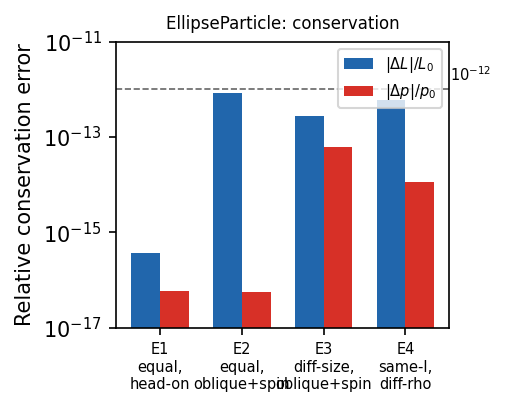
\includegraphics[width=\linewidth]{figures/ellipse_conservation.png}
  \caption{Angular and linear momentum conservation residuals for the four
    EllipseParticle collision configurations (Table~\ref{tab:ellipse}).
    All values lie below $10^{-12}$, establishing machine-precision
    conservation for arbitrary particle shape.}
  \label{fig:ellipse_conservation}
\end{figure}

\textbf{Contact forces and tangential coupling.}
The EPD contact model assigns the repulsive force to the nearest pair of
perimeter segments between two particles.  For a finite-$N$ perimeter, the
contact node does not sit exactly at the geometric point of closest approach,
so the force direction deviates slightly from the ideal surface normal.  The
ratio of tangential to normal impulse, $J_t/J_n$, measured from single-step
contact events~\cite{contactforce_code} ranges from 0.001 (near-normal impact,
$\theta = 15^\circ$) to 0.22 (oblique impact, $\theta = 45^\circ$) at $N = 32$.
This tangential coupling acts as effective \emph{micro-friction} even though
no friction law is imposed: it transfers a small fraction of translational
kinetic energy into spin during contact, giving a coefficient of restitution
$\text{COR} < 1$ even at zero damping ($\alpha_d = 0$).  The torque from
this tangential component is applied exactly by the integrator (torque error
$< 2 \times 10^{-15}$ relative), confirming that the effect is a genuine
physical feature of the discrete contact geometry, not a numerical artifact.
The magnitude decreases as $N^{-1/2}$ (fewer nodes span the contact arc at
larger $N$), and is negligible ($J_t/J_n < 0.01$) for $\theta < 20^\circ$
at $N \geq 32$.

\subsection{Perimeter regularization $k_{\rm reg}$: pseudo-force formulation
and discretization error}
\label{sec:kreg}

To prevent perimeter nodes from clustering or thinning during long
simulations, we add a soft \emph{spacing} pseudo-force at each node:
\begin{equation}
  \mathbf{F}_{\rm reg}[n] = k_{\rm reg}\,\frac{1}{2}(L^+_n - L^-_n)\,\hat{t}_n,
\label{eq:freg}
\end{equation}
where $L^+_n = |\mathbf{x}_{n+1} - \mathbf{x}_n|$ and
$L^-_n = |\mathbf{x}_n - \mathbf{x}_{n-1}|$ are the forward and backward
edge lengths at node $n$, and $\hat{t}_n$ is the bisector tangent
(average of the two adjacent edge unit tangents). Equation~(\ref{eq:freg})
pushes a node forward along the local perimeter direction when its
forward edge is longer, redistributing the spacing toward the equilibrium
$L^+ = L^-$ (uniform edge lengths).

\textbf{Non-conservativity.}
$\mathbf{F}_{\rm reg}$ is \emph{not} the gradient of any scalar potential.
Direct verification: the symmetry condition
$\partial F_{{\rm reg},i}/\partial x_j = \partial F_{{\rm reg},j}/\partial x_i$
required for $\mathbf{F}_{\rm reg} = -\nabla U_{\rm reg}$ fails for off-diagonal
node pairs. Consequently $\mathbf{F}_{\rm reg}$ does not strictly conserve
energy; the work it performs on a sliding node is not balanced against any
underlying $U_{\rm reg}$. In the damped physics integrator the
unaccounted work is dissipated by drag and is bounded well below
thermal-noise scale; in gradient-based optimization workflows used for
energy minimization or initial-condition preparation, the system simply
seeks the configuration where
$\mathbf{F}_{\rm phys} + \mathbf{F}_{\rm reg} = 0$ at every node, which
is well-posed independent of conservativity.

\textbf{Exclusion from rigid-body sums.}
Because $\sum_n \mathbf{F}_{\rm reg}[n]$ is generally non-zero for deformed
shapes (the per-node tangents weight the telescoping
$(L^+ - L^-)$ contributions inhomogeneously), including
$\mathbf{F}_{\rm reg}$ in the rigid-body resultants
Eq.~(\ref{eq:FT}) would impart spurious translation and rotation. The
implementation therefore excludes $\mathbf{F}_{\rm reg}$ from
$\mathbf{F}$ and $T$, applying it only to the elastic displacements
$\mathbf{u}_i$ in the co-moving frame. Rigid-body motion is driven only
by Newton-third-law-respecting forces (line tension, area pressure,
bending, contact, drag).

\textbf{Discretization artifact: straight-line slide vs.\ spline resample.}
The pseudo-force Eq.~(\ref{eq:freg}) slides node $n$ along its bisector
tangent $\hat{t}_n$. Geometrically this is a \emph{straight-line} translation
in space, whereas the ``true'' resample of node $n$ along the local
perimeter contour follows a curved path. For a node sitting on a smooth
arc with curvature $\kappa$, sliding along the tangent by $\Delta$
deviates from the arc by
\begin{equation}
  \delta \;\approx\; \frac{1}{2}\Delta^2 \kappa,
\label{eq:slide_error}
\end{equation}
in the inward normal direction (sagitta of an arc subtending arc length
$\Delta$). After the slide, the local curvature, outward normal, and
adjacent edge lengths at $n$ are all perturbed slightly, propagating
small errors into the bending, line tension, and contact terms.

A geometrically clean alternative would be to fit a local quadratic
or cubic spline through $\{\mathbf{x}_{n-1}, \mathbf{x}_n, \mathbf{x}_{n+1}\}$,
locate the equispaced arclength position $s_n^* = (s_{n-1}+s_{n+1})/2$
on the spline, and set $\mathbf{x}_n' = \mathbf{C}(s_n^*)$. This is
exactly on-contour by construction. We do not implement this because
(i) the magnitude of the artifact is small at typical simulation
parameters (see below), and (ii) a position-update operator does not
fit the unified force-based abstraction shared by the physics integrator,
the rigid-body decomposition, and the gradient-based optimizers.

\textbf{Magnitude estimate.}
The per-step displacement $\Delta$ from $k_{\rm reg}$ depends on context:
in the physics integrator at typical $\alpha_d \cdot dt = 0.2$ and
near-equispaced configurations, $\Delta \lesssim 10^{-4}\,L_0$; in
gradient optimizers (\textsc{adam} at lr $= 10^{-3}$, \textsc{fire}
with $dt_{\max} = 0.03$), $\Delta \lesssim 10^{-3}\,L_0$. We consider
two limiting curvature regimes spanning the expected range
encountered in dense deformable packings:

\begin{itemize}
\item \emph{Free perimeter arch under modest pressure} —
$\kappa \approx 1/(2R_0)$. The arch bulges slightly outward from the
reference circle; most of the resampling error accumulates here.

\item \emph{Contact patch} — $\kappa \approx 0$. The perimeter is nearly
straight along the contact arc; sliding along the tangent stays on the
chord. Effectively zero artifact.
\end{itemize}

A third regime occupies a small set of nodes:

\begin{itemize}
\item \emph{Contact-free transition node} — at the boundary between a
contact arc and a free patch the local effective curvature can be
$\kappa \sim 1/L_0 \approx N/(2\pi R_0)$ over a single edge, producing
the largest per-step artifact in the system.
\end{itemize}

Substituting $\Delta = 10^{-3}$ length units into Eq.~(\ref{eq:slide_error})
gives the per-step deviations summarized in Table~\ref{tab:kreg_error}.
The cumulative steady-state deviation is bounded by the elastic restoring
force timescale $\tau_{\rm restore}$ over which line tension snaps the
off-curve node back: $\delta_{\rm steady} \approx
\delta_{\rm step} \cdot \tau_{\rm restore}/\Delta t$, typically a few
hundred times the per-step value.

\begin{table}[htb]
\caption{Per-step and steady-state off-contour deviation from
straight-line $k_{\rm reg}$ slide vs.\ exact spline resample, at
$\Delta = 10^{-3}\,L_0$ per step (typical optimizer regime).
The artifact is concentrated at the small fraction of nodes living
on contact-free transition boundaries, which coincide with the
\emph{stuck} nodes identified by the per-node force diagnostics.}
\label{tab:kreg_error}
\begin{ruledtabular}
\begin{tabular}{lccl}
  Region & Curvature $\kappa$ & $\delta_{\rm step}$ & $\delta_{\rm steady}$ \\
\hline
  Free arch interior (modest pressure)
    & $1/(2R_0) \approx 0.5$
    & $2.5 \times 10^{-7}$
    & $\sim 10^{-5}$ \\
  Contact patch interior
    & $\approx 0$
    & $0$
    & $0$ \\
  Contact-free transition node
    & $\sim 1/L_0 \approx 10$
    & $5 \times 10^{-6}$
    & $\sim 10^{-3}$ \\
\end{tabular}
\end{ruledtabular}
\end{table}

\textbf{Practical implications.}
For dynamic shear or hopper simulations with drive forces of order
$10^{-2}$--$10^{-1}$, the regularization artifact is several orders of
magnitude below noise. For initial-condition preparation in jammed
packings, where one may push $\|F\|_\infty$ below $10^{-3}$, the
contribution from contact-free transition nodes becomes comparable to
the achievable floor and contributes meaningfully to the \emph{stuck}
set identified by per-node force diagnostics. Reducing $k_{\rm reg}$
suppresses the artifact at the cost of slower equispacing maintenance;
adopting a spline-based resample operator would eliminate it at the
cost of a position-update step outside the force-flow abstraction.

\subsection{Decoupled $k_{\rm reg}$ integration: position-only update}
\label{sec:kreg_decouple}

The pseudo-force formulation of Eq.~(\ref{eq:freg}) has a subtle dynamical
side effect that becomes visible when one looks at force vectors at the
node level. Because $\mathbf{F}_{\rm reg}$ enters the equations of motion
as a force, it contributes to the elastic-node velocity $\dot{\mathbf{u}}$
and hence to the lab-frame node velocity $\mathbf{v}_{\rm node}$. The
per-node Stokes drag kernel,
\begin{equation}
  \mathbf{f}_{\rm drag}[n] \;=\; -\xi\, \mathbf{v}_{{\rm node},n}\,\Delta L_n,
\label{eq:fdrag_kreg}
\end{equation}
then acts on the $k_{\rm reg}$-driven tangential motion, generating a
spurious drag force that opposes the resampling slide. Two artifacts
follow.

\begin{enumerate}
\item \emph{Off-bisector residual in $\mathbf{F}_{\rm phys}$.} For an
emulsion droplet ($E_t = 0$, $EI = 0$ by construction; see
Sec.~\ref{sec:kreg}), the only physical perimeter forces are line tension
$\gamma$ and area pressure $K_A$. Both project strictly along the local
angle bisector. Per-node visualization of
$\mathbf{F}_{\rm phys} \equiv \mathbf{F}_{\rm total} - \mathbf{F}_{\rm reg}$
on a quenched packing therefore should show vectors aligned with the
bisector to machine precision. In the original formulation, however,
$\mathbf{F}_{\rm phys}$ exhibits off-bisector components on free arcs of
order $\xi \cdot v_{\rm reg}$. These trace directly to drag acting on
$k_{\rm reg}$-induced tangential velocity, not to any physical force.

\item \emph{Weak rotational drive on contacting particles.}
Asymmetric contact configurations produce asymmetric tangential motion
patterns around the perimeter; the resulting drag torque is small but
nonzero. Because $\beta_{\rm rb}$ damps rigid-body rotation, the spin-up
saturates quickly, but the mechanism injects a small unphysical
chirality into the dynamics. By symmetry and angular-momentum
conservation, a real emulsion droplet at rest (no Marangoni or external
flow) exhibits no spontaneous rotation; the $k_{\rm reg}$/drag coupling
is the source of this artifact in the discrete model.
\end{enumerate}

The root cause is treating a parameterization device as physical motion:
$k_{\rm reg}$ slides node \emph{labels} along the perimeter to maintain
even discretization, but the underlying continuous interface is at rest.
Stokes drag should be insensitive to this label-sliding, and is so only
when we remove $k_{\rm reg}$ from the integrated velocity.

We resolve this by treating $k_{\rm reg}$ as a per-step position
projection rather than a force entering Newton's equations. The semi-implicit
elastic update becomes
\begin{equation}
  \dot{\mathbf{u}}_{\rm new}
    \;=\; \frac{\dot{\mathbf{u}} + \mathbf{a}_{\rm phys}\,\Delta t}
              {1 + \alpha\,\Delta t},
  \qquad
  \mathbf{a}_{\rm phys}
    \;=\; \frac{1}{m_{\rm node}}
          \!\Big(\mathbf{f}_{\rm phys} - \tfrac{1}{N}\!\sum_n \mathbf{f}_{\rm phys}[n]\Big),
\label{eq:udot_decoupled}
\end{equation}
where $\mathbf{f}_{\rm phys} = \mathbf{f}_{\rm el} + \mathbf{f}_{\rm contact}
+ \mathbf{f}_{\rm drag}$ excludes $\mathbf{f}_{\rm reg}$.
The position update then adds the per-step regularization slide as an
instantaneous, non-momentum-bearing translation:
\begin{equation}
  \mathbf{u}_{\rm new}
    \;=\; \mathbf{u} + \dot{\mathbf{u}}_{\rm new}\,\Delta t
        + \mathbf{v}_{\rm reg}\,\Delta t,
  \qquad
  \mathbf{v}_{\rm reg}
    \;\equiv\; \mathbf{f}_{\rm reg}/m_{\rm node}.
\label{eq:u_decoupled}
\end{equation}
The drag kernel of Eq.~(\ref{eq:fdrag_kreg}) sees $\mathbf{v}_{\rm node}$
built from $\dot{\mathbf{u}}_{\rm new}$ (without $k_{\rm reg}$
contribution), so no spurious drag is generated by the parameterization
slide. The non-conservativity of $\mathbf{F}_{\rm reg}$ becomes explicit:
it is a per-step constraint enforcement, not a force requiring an energy
account.

\textbf{Validation.} The decoupled formulation is enabled by default; the
legacy integrate-as-force formulation is preserved as an opt-in flag
(\texttt{decouple\_kreg = False}) for backward reproducibility. We verified:
\begin{enumerate}
\item \emph{Bit-exactness in legacy mode.} With the flag off, a 5000-step
quench from a saved post-swell configuration ($\phi=0.86$, $P=16$,
$\alpha = 0.01/dt$, $\beta_{\rm rb} = 0.5/dt$) reproduces the pre-change
trajectory exactly ($\max|\Delta\mathbf{x}| = 0$ at every recorded frame).
\item \emph{Stability in decoupled mode.} The same quench with the flag on
remains stable and bounded; the trajectory diverges smoothly from the
legacy one as expected from the modified drag coupling, reaching
$\|F\|_\infty = 6.8 \times 10^{-3}$ (vs.\ $4.7 \times 10^{-3}$ legacy).
\item \emph{Swell convergence preserved.} A full adaptive swell from
$\phi = 0.49$ to $\phi = 0.86$ converges in both formulations, with the
decoupled formulation reaching $\sim 40\%$ lower residual
$\|F\|_\infty$ at the target density (the legacy formulation carries
extra residual stress from the spurious tangential drag coupling).
\item \emph{Force-bisector alignment.} For an isolated emulsion droplet
with a small radial perturbation, the decoupled formulation produces
$\mathbf{F}_{\rm phys}$ vectors aligned with the angle bisector at every
node to machine precision throughout a 60-step dynamic run, recovering
the analytic structure $\mathbf{F}_{\rm phys} = \gamma(\hat{t}_+ - \hat{t}_-)
+ P\,L_0\,\hat{n}_{\rm node}$.
\end{enumerate}

%%============================================================
\section{Dimensional Analysis and Parameter Reduction}
\label{sec:dimanalysis}
%%============================================================

\subsection{$S$ as a pure force scale}

We introduce a force scale $S$ via the membrane stiffness at $R_0 = 1$:
$\Elb \equiv 12S/\tau^2$.  For a disk of radius $R_0$, the simulator uses
$\Elc = \Elb R_0$.  The thin-shell bending stiffness then gives
\begin{equation}
  EI = \Elc \frac{(\tau R_0)^2}{12}
     = \frac{12S}{\tau^2} R_0 \frac{\tau^2 R_0^2}{12} = S R_0^3.
\label{eq:EI}
\end{equation}
All dimensionless observables are independent of $S$: sweeping $S$ over
$\{0.01, 0.1, 1.0, 10\}$ (1000$\times$ range) gives $\cv = 0.00\%$ for
$\dA$ and $\numes$.  We fix $S = 1$.

\subsection{$R_0$ as a pure length scale}

All dimensionless observables are independent of $R_0$ when parameters scale as:
\begin{equation}
  EI = SR_0^3, \qquad \Karea = q\,\Elb, \qquad C = C_0 S(1 + q),
\label{eq:R0scaling}
\end{equation}
where $\Karea$ and $C$ are held \emph{constant} (not scaled with $R_0$).
The scaling argument: bending force per node $\sim EI/R_0^2 \propto R_0$;
membrane force $\sim \Elc \propto R_0$; area force $\sim \Karea L_0 \propto R_0$
(constant $\Karea$); contact force $\sim C g \propto R_0$ (since $g \propto R_0$
geometrically).  All force ratios are therefore $R_0$-independent.  We fix
$R_0 = 1$ for calibration; the recipe (Sec.~\ref{sec:recipe}) applies the correct
scalings for $R_0 \neq 1$.

\subsection{Two dimensionless physical parameters}

With $S = R_0 = 1$, the model reduces to two parameters:

\textbf{Bending number} $b = EI/\Elc|_{R_0=1} = \tau^2/12$: ratio of bending to
membrane stiffness at the calibration geometry.

\textbf{Area stiffness ratio} $q = \Karea/\Elb$: ratio of area penalty to
membrane stiffness at $R_0 = 1$.  Because $\Karea$ is constant, $q$ is genuinely
$R_0$-independent.

\textbf{Natural midpoint $q \cdot b = 1$:}
\begin{equation}
  q \cdot b = \frac{\Karea \cdot EI}{\El^2} = 1
\label{eq:midpoint}
\end{equation}
is the locus where area and bending stiffness are balanced at the membrane scale.
At the working point $b = 0.2$, this occurs at $q = 5$.

%%============================================================
\section{Numerical Calibration}
\label{sec:numcalib}
%%============================================================

\subsection{Contact stiffness $C$}

The contact force must dominate both the membrane and area-spring restoring forces:
\begin{equation}
  C \gtrsim S(1 + q).
\label{eq:Ccrit}
\end{equation}
Crucially, $C$ must be $\tau$-independent (since $EI = S$ is $\tau$-independent),
while $\El \propto 1/\tau^2$.  An earlier parameterization $C \propto \El$ gave
cc $= 22\%$ overlap at $\tau = 0.20$.  A bisection sweep over $C_0 = C/[S(1+q)]$
at $\tau \in \{0.05, 0.10, 0.20\}$ and $q \in \{0.1, 1, 5, 10\}$, requiring
contact compression cc $< 2\%$, yields:
\begin{equation}
  \boxed{C = 3000\,S\,(1 + q).}
\label{eq:C}
\end{equation}

\subsection{Damping parameter}
\label{sec:damp_calib}

\textit{Background: elastic mode spectrum.}
The EPD shell supports two distinct families of in-plane elastic modes.
Fast \emph{extensional} (membrane) modes involve changes in arc length;
their characteristic frequency is set by the edge-wave speed,
$\omega_\text{ext} \sim 2c_\text{edge}/R_0$ with
$c_\text{edge} = \sqrt{E_l R_0/(\rho_l L_0)}$.
At the reference parameters ($\tau = 0.2$, $R_0 = 1$, $N = 32$)
this gives $\omega_\text{ext} \approx 78$\,rad\,s$^{-1}$.
Slow \emph{inextensional bending} modes preserve arc length to leading
order; their restoring force comes from the bending stiffness $EI = SR_0^3$.
These are the Euler--Bernoulli ring modes~\cite{Soedel2004}, with
frequency~\cite{Wah1962}
\begin{equation}
  \omega_n = \frac{n(n^2-1)}{\sqrt{n^2+1}}
    \sqrt{\frac{EI}{\rho_l R_0^4}}.
\label{eq:ring_bend}
\end{equation}
For the dominant $n = 2$ (elliptical squish) mode, with
$EI = SR_0^3$ and $\rho_l = \rho_f \tau R_0$:
\begin{equation}
  \omega_{2,\text{bend}} = \frac{6}{\sqrt{5}}
    \sqrt{\frac{S}{\rho_f\,\tau\,R_0^2}}.
\label{eq:omega2bend}
\end{equation}
At reference parameters this gives $\omega_{2,\text{bend}} = 6.0$\,rad\,s$^{-1}$,
roughly 13$\times$ slower than the extensional modes.

\textit{Why bending modes dominate post-collision ringing.}
A head-on collision compresses the disk into an approximately elliptical shape,
strongly projecting onto the $n = 2$ bending mode.  The extensional modes are
excited equally (all modes receive the same force amplitude per Fourier component)
but contribute displacements $\sim \omega_n^{-2}$ times smaller.  Since
$(\omega_\text{ext}/\omega_{2,\text{bend}})^2 \approx 170$, the observable
post-collision shape oscillation is dominated by the bending mode.  A direct
measurement confirms this: after a two-disk head-on collision at $v_0 = 2$
with $\alpha_d = 0.5$, an FFT of the post-separation node-0 radial displacement
gives $\omega_\text{ring} = 6.0002$\,rad\,s$^{-1}$, within 0.003\% of
Eq.~(\ref{eq:omega2bend})~\cite{dampcalib_code}.

\textit{Amplitude decay law.}
The damping term $-\alpha_d \dot{\mathbf{u}}_i$ in
Eq.~(\ref{eq:verlet}) gives, for any underdamped mode (quality factor
$Q = \omega_n/\alpha_d > 1$), a universal amplitude
e-folding time
\begin{equation}
  T_\text{decay} = \frac{2}{\alpha_d},
\label{eq:Tdecay}
\end{equation}
independent of mode frequency or stiffness.  This is verified
numerically~\cite{dampcalib_code} to $< 0.1\%$ for $Q \geq 1.2$.
For overdamped modes ($Q < 1$), the decay slows to
$T_\text{actual} \approx \alpha_d/\omega_{2,\text{bend}}^2 > 2/\alpha_d$.

\textit{Scaling verification.}
Equation~(\ref{eq:omega2bend}) is verified by free-vibration tests
across seven parameter combinations (Table~\ref{tab:damp_scaling} and
Fig.~\ref{fig:bending_cor}a).  The measured bending frequency agrees
with theory to $< 2\%$ in all cases, confirming the independent
$1/\sqrt{\tau}$, $1/R_0$, and $\sqrt{S}$ scalings~\cite{dampcalib_code}.

\begin{table}[htb]
\caption{Bending-mode scaling verification at $N = 32$.
  $\alpha_d = 0.5$ throughout.  All errors $< 2\%$.}
\label{tab:damp_scaling}
\begin{ruledtabular}
\begin{tabular}{lrrl}
  Parameters & $\omega_{2,\text{theory}}$ & $\omega_{2,\text{meas}}$ & error \\
\hline
  $\tau{=}0.05,\,R_0{=}1,\,S{=}1$ & 12.000 & 12.193 & $+1.6\%$ \\
  $\tau{=}0.10,\,R_0{=}1,\,S{=}1$ &  8.485 &  8.484 & $-0.0\%$ \\
  $\tau{=}0.20,\,R_0{=}1,\,S{=}1$ &  6.000 &  5.945 & $-0.9\%$ \\
  $\tau{=}0.20,\,R_0{=}0.5,\,S{=}1$ & 12.000 & 11.968 & $-0.3\%$ \\
  $\tau{=}0.20,\,R_0{=}2.0,\,S{=}1$ &  3.000 &  2.960 & $-1.3\%$ \\
  $\tau{=}0.20,\,R_0{=}1,\,S{=}0.1$ &  1.897 &  1.864 & $-1.8\%$ \\
  $\tau{=}0.20,\,R_0{=}1,\,S{=}4.0$ & 12.000 & 11.898 & $-0.9\%$ \\
\end{tabular}
\end{ruledtabular}
\end{table}

\textit{COR--damping tradeoff.}
A key consequence of Eq.~(\ref{eq:ring_bend}) is that the contact duration
$T_\text{contact}$ is comparable to the bending period: at reference parameters
$T_\text{contact} \approx 1.57$\,s $\approx 1.5\,T_{2,\text{bend}}$.  The
bending mode resonates \emph{during} contact.  As a result, the coefficient
of restitution depends strongly on $\alpha_d$ (Table~\ref{tab:cor_alpha} and
Fig.~\ref{fig:bending_cor}b): low $\alpha_d$ gives high COR but persistent
ringing; high $\alpha_d$ suppresses ringing but dissipates energy during contact.
This is a genuine \emph{physical design tradeoff}, not a numerical artifact.

\begin{table}[htb]
\caption{COR vs.\ $\alpha_d$ at reference parameters
  ($\tau = 0.20$, $R_0 = 1$, $N = 32$, $S = 1$, $v_0 = 0.5$, $C = 3000$).
  $Q = \omega_{2,\text{bend}}/\alpha_d$.}
\label{tab:cor_alpha}
\begin{ruledtabular}
\begin{tabular}{rrrll}
  $\alpha_d$ & $Q$ & $T_\text{decay}$ & COR & Ringing character \\
\hline
    0.3 & 20.0 & 6.67 & 0.894 & persistent ($>$10 cycles) \\
    0.5 & 12.0 & 4.00 & 0.868 & persistent \\
    1.0 &  6.0 & 2.00 & 0.825 & persistent \\
    2.0 &  3.0 & 1.00 & 0.729 & few cycles \\
    3.0 &  2.0 & 0.67 & 0.662 & few cycles \\
    6.0 &  1.0 & 0.33 & 0.530 & no visible ringing \\
   10.0 &  0.6 & 0.20 & 0.417 & overdamped \\
   20.0 &  0.3 & 0.10 & 0.289 & overdamped \\
\end{tabular}
\end{ruledtabular}
\end{table}

\begin{figure}[htb]
  \centering
  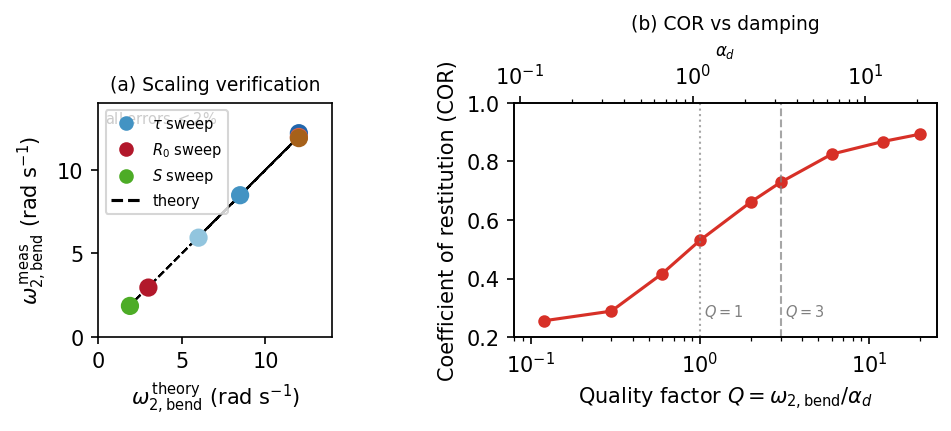
\includegraphics[width=\linewidth]{figures/bending_mode_and_cor.png}
  \caption{%
    \textbf{(a)} Bending-mode scaling verification: measured $\omega_{2,\text{bend}}$
    vs.\ theory (Eq.~\ref{eq:omega2bend}) across seven parameter combinations
    spanning $\tau$, $R_0$, and $S$ (all errors $< 2\%$).
    \textbf{(b)} Coefficient of restitution (COR) vs.\ quality factor
    $Q = \omega_{2,\text{bend}}/\alpha_d$ at reference parameters.
    The strong $\alpha_d$-dependence reflects that $T_\text{contact} \approx
    1.5\,T_{2,\text{bend}}$: the bending mode resonates during contact.
    The vertical dashed and dotted lines mark $Q = 3$ (current default,
    COR $= 0.73$) and $Q = 1$ (no visible ringing, COR $= 0.53$).%
  }
  \label{fig:bending_cor}
\end{figure}

\textit{Design formula and calibration choice.}
The general recipe for choosing $\alpha_d$ given a target quality factor
$Q_\text{target}$ is:
\begin{equation}
  \alpha_d = \frac{\omega_{2,\text{bend}}}{Q_\text{target}}
           = \frac{6}{\sqrt{5}}\,
             \frac{\sqrt{S/(\rho_f\,\tau)}}{Q_\text{target}\,R_0}.
\label{eq:alpha_design}
\end{equation}
In dimensionless form, defining
$\tilde\alpha = \alpha_d R_0\sqrt{\rho_f\tau/S}\cdot\sqrt{5}/6$:
critical damping ($Q = 1$) corresponds to $\tilde\alpha = 1$ for all
parameter combinations.

For the quasi-static two-disk calibration (Sec.~\ref{sec:calib}), the
choice is constrained differently: $\alpha_d$ must damp transient elastic
oscillations within a few loading steps, but must not over-damp the
low-$q$ response.  A sweep over $\alpha_d \in \{0.5, 1.0, 1.5, 2.0, 3.0, 5.0\}$
requiring kinetic energy $< 10^{-4}$ of strain energy within $\sim 10$
wave periods gives
\begin{equation}
  \boxed{\alpha_d = \alpha_0 / T_\text{wave} = 2.0,
    \quad (\zeta \approx 16\%, \; Q \approx 3).}
\label{eq:alpha0}
\end{equation}
At this value, $\alpha_d < 1.0$ produces oscillation artifacts in
$\numes(\ep)$; $\alpha_d > 3.0$ artificially stiffens the low-$q$ response.
For free-flight multi-particle simulations, Eq.~(\ref{eq:alpha_design})
should be used directly to match the desired COR and ringing character
(Table~\ref{tab:cor_alpha}).

%%============================================================
\section{Phase-Space Structure}
\label{sec:phasespace}
%%============================================================

\subsection{Calibration geometry}

All calibration uses a single canonical geometry: two identical EPD disks squeezed
symmetrically between two rigid horizontal walls, with centers initially separated
by $2R_0$ (touching, zero overlap).  No side walls: particles expand laterally
without constraint.  Observables at reference strain $\eref$:
\begin{align}
  \dA(\%) &= \bigl(1 - A/A_0\bigr) \times 100,
  \label{eq:dA}\\
  \numes &= -\varepsilon_{\rm lat}/\varepsilon_{\rm vert}.
  \label{eq:nu}
\end{align}
In 2D, $\numes = 1$ for an incompressible disk and $\numes = 0$ for one that
does not expand laterally.

\subsection{Shape collapse}

A central result is that the perimeter \emph{shape} at given $\dA$ is independent
of the individual parameters $(\El, EI, \Karea)$.  Writing the combined elastic
energy as $E_{\rm mem} + E_{\rm bend} = \Elc \cdot \mathcal{F}_b(\{\mathbf{x}_i\})$,
the prefactor $\Elc$ cancels from the Euler--Lagrange equations: the minimizing
shape depends only on $b$ and geometric constraints, not on $\El$, $\tau$, $S$,
or $q$ individually.  Differences in perimeter shapes across $q$ at fixed $\ep$
arise entirely from different $\dA$ values, not different shapes at the same $\dA$.
The shape collapse is demonstrated visually in Fig.~\ref{fig:sweep_and_shapes}
(bottom) and in Movies~S2--S6.

\subsection{One-to-one relationship between $\dA$ and $\numes$}

Figure~\ref{fig:sweep_and_shapes} (top) shows the calibration curves
$\numes(q)$ and $\dA(q)$ at $b = 0.2$.  Both are monotone: as $q$ increases,
$\dA$ decreases and $\numes$ increases.  The one-to-one relationship
$(\dA, \numes)(q)$, shown in Fig.~\ref{fig:dA_nu_trajectory}, confirms that
specifying either observable at fixed $b$ uniquely determines the other.  The
model therefore exposes a genuine one-parameter squishiness axis.

Movie~S1 provides a side-by-side comparison across the full squishiness range;
Movies~S2--S6 show individual $q$ values in detail.

\begin{figure*}[t]
  \centering
  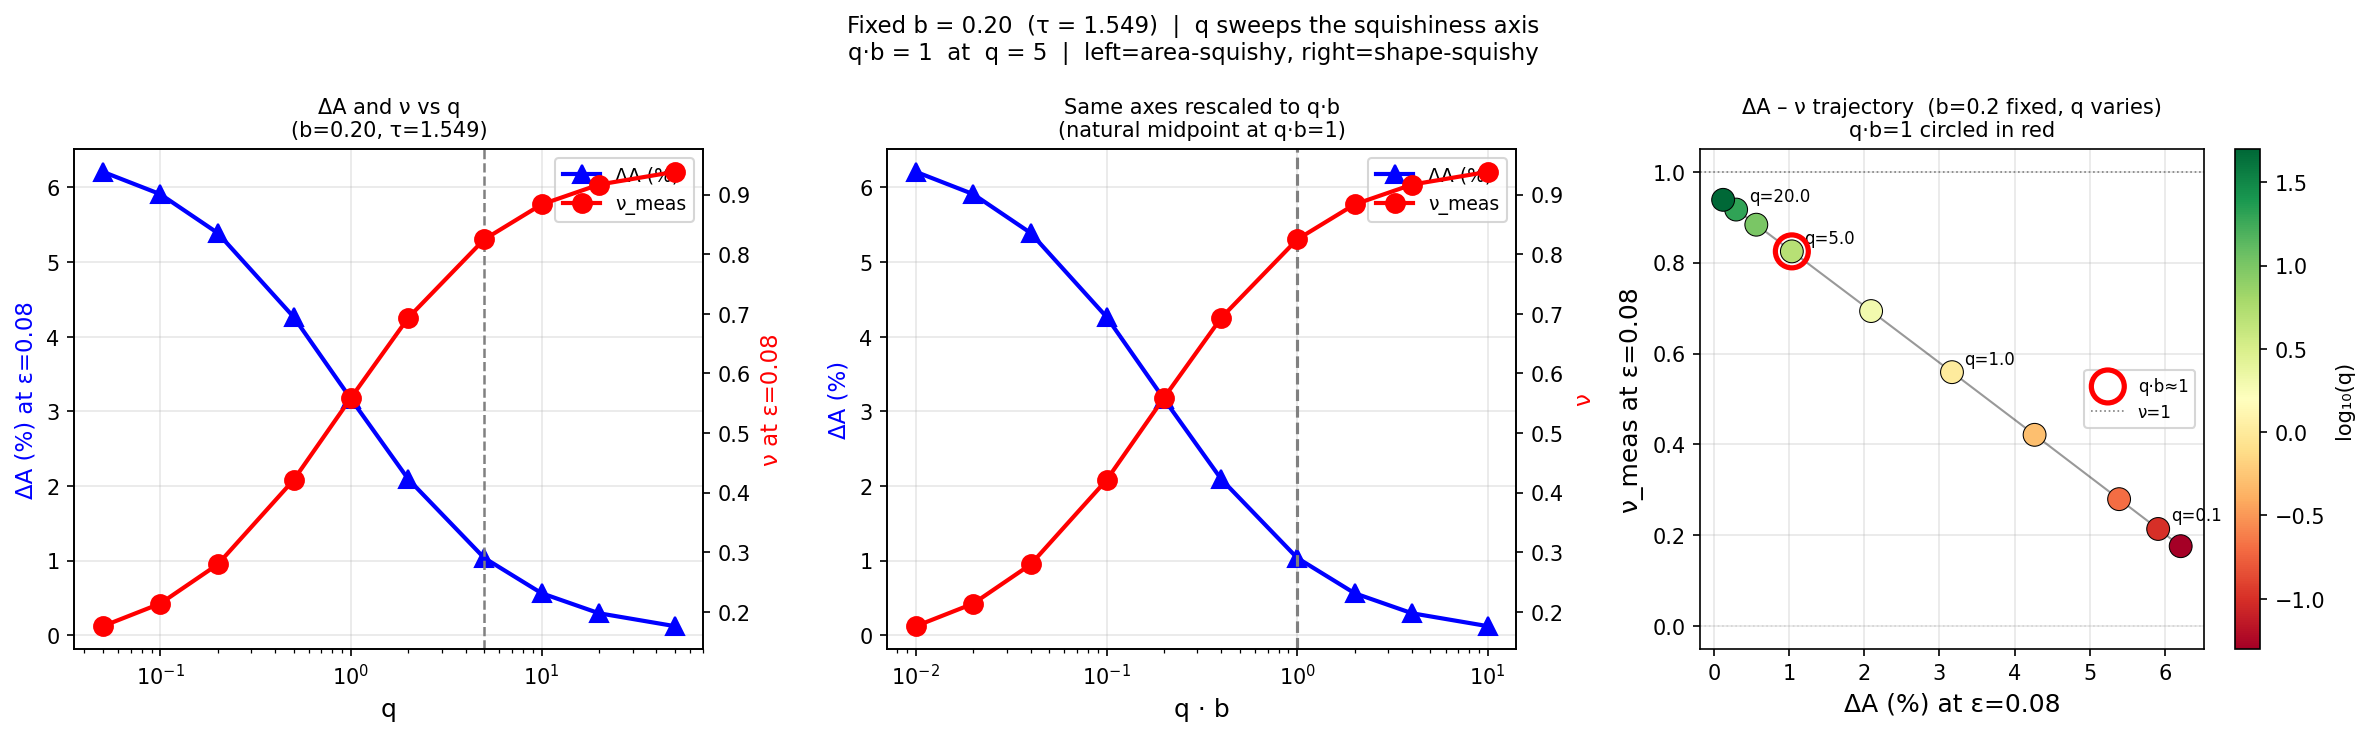
\includegraphics[width=0.68\linewidth]{figures/fixed_b_sweep.png}\\[4pt]
  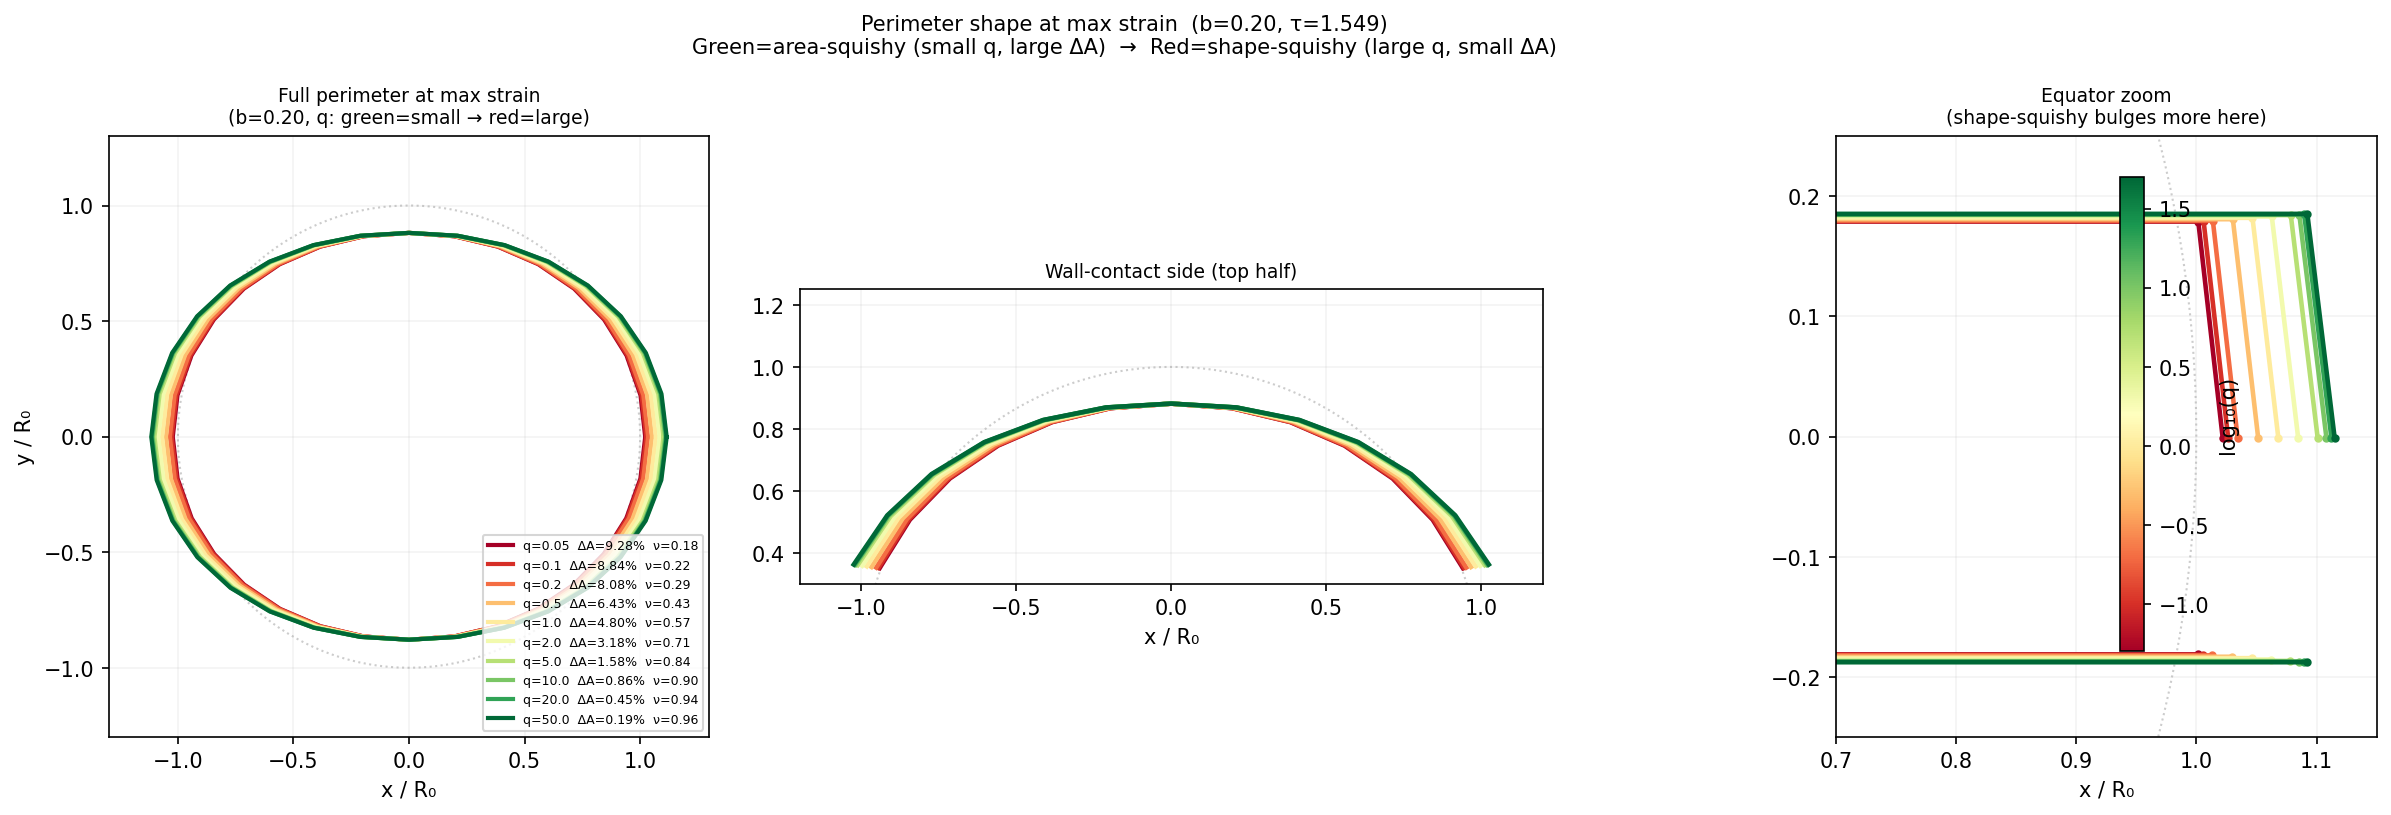
\includegraphics[width=0.68\linewidth]{figures/perimeter_overlay.png}
  \caption{%
    \textbf{Top:} Squishiness axis at fixed $b = 0.2$: $\numes$ (filled circles,
    left axis) and $\dA$ (open squares, right axis) vs.\ $q$ at $\eref = 0.08$.
    The vertical dashed line marks the midpoint $q \cdot b = 1$ ($q = 5$).
    \textbf{Bottom:} Shape collapse.  Centered perimeter outlines at maximum
    strain ($\ep \approx 0.12$) overlaid for $q \in \{0.05, 0.5, 1, 5, 20, 50\}$
    (blue to red with increasing $q$).  At fixed $\dA$, all outlines lie on a
    single curve; the visible differences arise entirely from different $\dA$
    values.  See Movie~S1 for the animated version.
  }
  \label{fig:sweep_and_shapes}
\end{figure*}

\begin{figure}[htb]
  \centering
  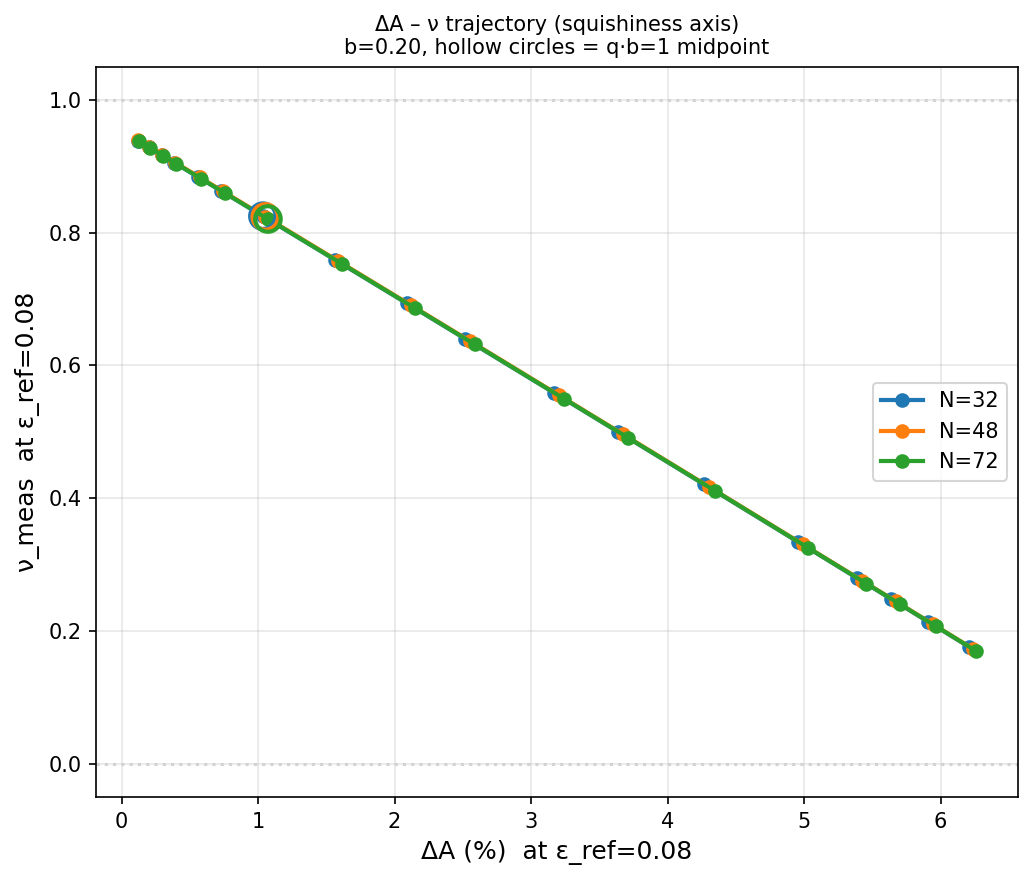
\includegraphics[width=\linewidth]{figures/calib_dA_nu_trajectory.png}
  \caption{%
    Trajectory in the $(\dA, \numes)$ plane as $q$ varies from 0.05 to 50 at
    $b = 0.2$, $\eref = 0.08$, $N = 48$.  The monotone curve demonstrates the
    one-to-one relationship between area loss and Poisson ratio at fixed $b$.
    Selected $q$ values are labeled; the midpoint $q \cdot b = 1$ is starred.
  }
  \label{fig:dA_nu_trajectory}
\end{figure}

%%============================================================
\section{Squishiness Axis: Calibration at $b = 0.2$}
\label{sec:calib}
%%============================================================

\subsection{Working point and calibration table}

Fixing $b = 0.2$ ($\tau \approx 1.549$) gives a clean squishiness sweep over
three decades of $q$.  The full 18-point calibration at $N = 48$, $\eref = 0.08$
is given in Table~\ref{tab:calib18}.

\begin{table}[htb]
\caption{Calibration table at $b = 0.2$, $N = 48$, $\eref = 0.08$.
  Boldface marks the midpoint $q \cdot b = 1$.}
\label{tab:calib18}
\begin{ruledtabular}
\begin{tabular}{rrrlr}
  $q$ & $q\cdot b$ & $\numes$ & $\dA$ (\%) & Character \\
\hline
  0.050 & 0.010 & 0.173 & 6.24 & area-compressible \\
  0.100 & 0.020 & 0.211 & 5.94 & area-compressible \\
  0.150 & 0.030 & 0.245 & 5.67 & area-compressible \\
  0.200 & 0.040 & 0.276 & 5.43 & area-compressible \\
  0.300 & 0.060 & 0.330 & 4.99 & compressible \\
  0.500 & 0.100 & 0.417 & 4.31 & compressible \\
  0.750 & 0.150 & 0.496 & 3.67 & compressible \\
  1.000 & 0.200 & 0.555 & 3.20 & intermediate \\
  1.500 & 0.300 & 0.637 & 2.55 & intermediate \\
  2.000 & 0.400 & 0.691 & 2.12 & intermediate \\
  3.000 & 0.600 & 0.758 & 1.59 & shape-deformable \\
  \textbf{5.000} & \textbf{1.000} & \textbf{0.824} & \textbf{1.05} & \textbf{midpoint} \\
  7.500 & 1.500 & 0.862 & 0.74 & shape-deformable \\
  10.00 & 2.000 & 0.883 & 0.57 & shape-deformable \\
  15.00 & 3.000 & 0.906 & 0.39 & shape-deformable \\
  20.00 & 4.000 & 0.917 & 0.30 & nearly incomp.\ \\
  30.00 & 6.000 & 0.929 & 0.20 & nearly incomp.\ \\
  50.00 & 10.00 & 0.939 & 0.12 & nearly incomp.\ \\
\end{tabular}
\end{ruledtabular}
\end{table}

\subsection{Sensitivity to $\eref$ and $N$}

Figure~\ref{fig:Nsensitivity} shows the calibration curves at
$N \in \{32, 48, 72, 120, 240\}$ (top) and
$\eref \in \{0.04, 0.06, 0.08, 0.10, 0.12\}$ (bottom).

\textit{N-sensitivity:} Extending the sweep to $N \in \{32, 48, 72, 120, 240\}$
reveals a systematic, monotone drift of the calibration curve toward lower $\numes$
at fixed $q$ as $N$ increases (Table~\ref{tab:Ndrift} and Fig.~\ref{fig:Ndrift}).
Within the low-resolution band $N \in \{32, 48, 72\}$ the drift remains modest:
$\Delta\numes^{\max} = 0.010$ (at $q = 0.75$).  However, extending to the
production tier $N = 240$ reveals a much larger cumulative shift:
$\Delta\numes^{\max} = 0.046$ (at $q = 1.0$), with $\Delta\numes > 0.02$ across
the entire mid-range $q \in [0.3, 10]$.

The physical origin of this drift is the same as the $1/N$ correction to the
contact force exponent discussed in Section~\ref{sec:contactlaw}: at smaller $N$
the discrete contact sum over perimeter nodes overestimates the Poisson ratio
because the bending-to-stretching coupling is resolved on a coarser arc.

\textit{Practical implication:} The calibration table (Table~\ref{tab:calib18},
at $N = 48$) is accurate to $|\Delta\numes| < 0.01$ for $N \leq 72$, but
\emph{must be recomputed at the target resolution} for production work at
$N = 240$.  Table~\ref{tab:calib240} gives the $N = 240$, $\eref = 0.08$ calibration.

\textit{$\eref$-sensitivity:} The maximum drift across $\eref \in \{0.04, 0.12\}$
is $\Delta\numes = 0.045$ at large $q$; the median is $0.033$.  The monotone
increase with $\eref$ is a quasi-static loading artefact: area-penalty
equilibration is incomplete at early strains.  The working point $\eref = 0.08$
balances contact development against quasi-linearity.

\begin{figure*}[t]
  \centering
  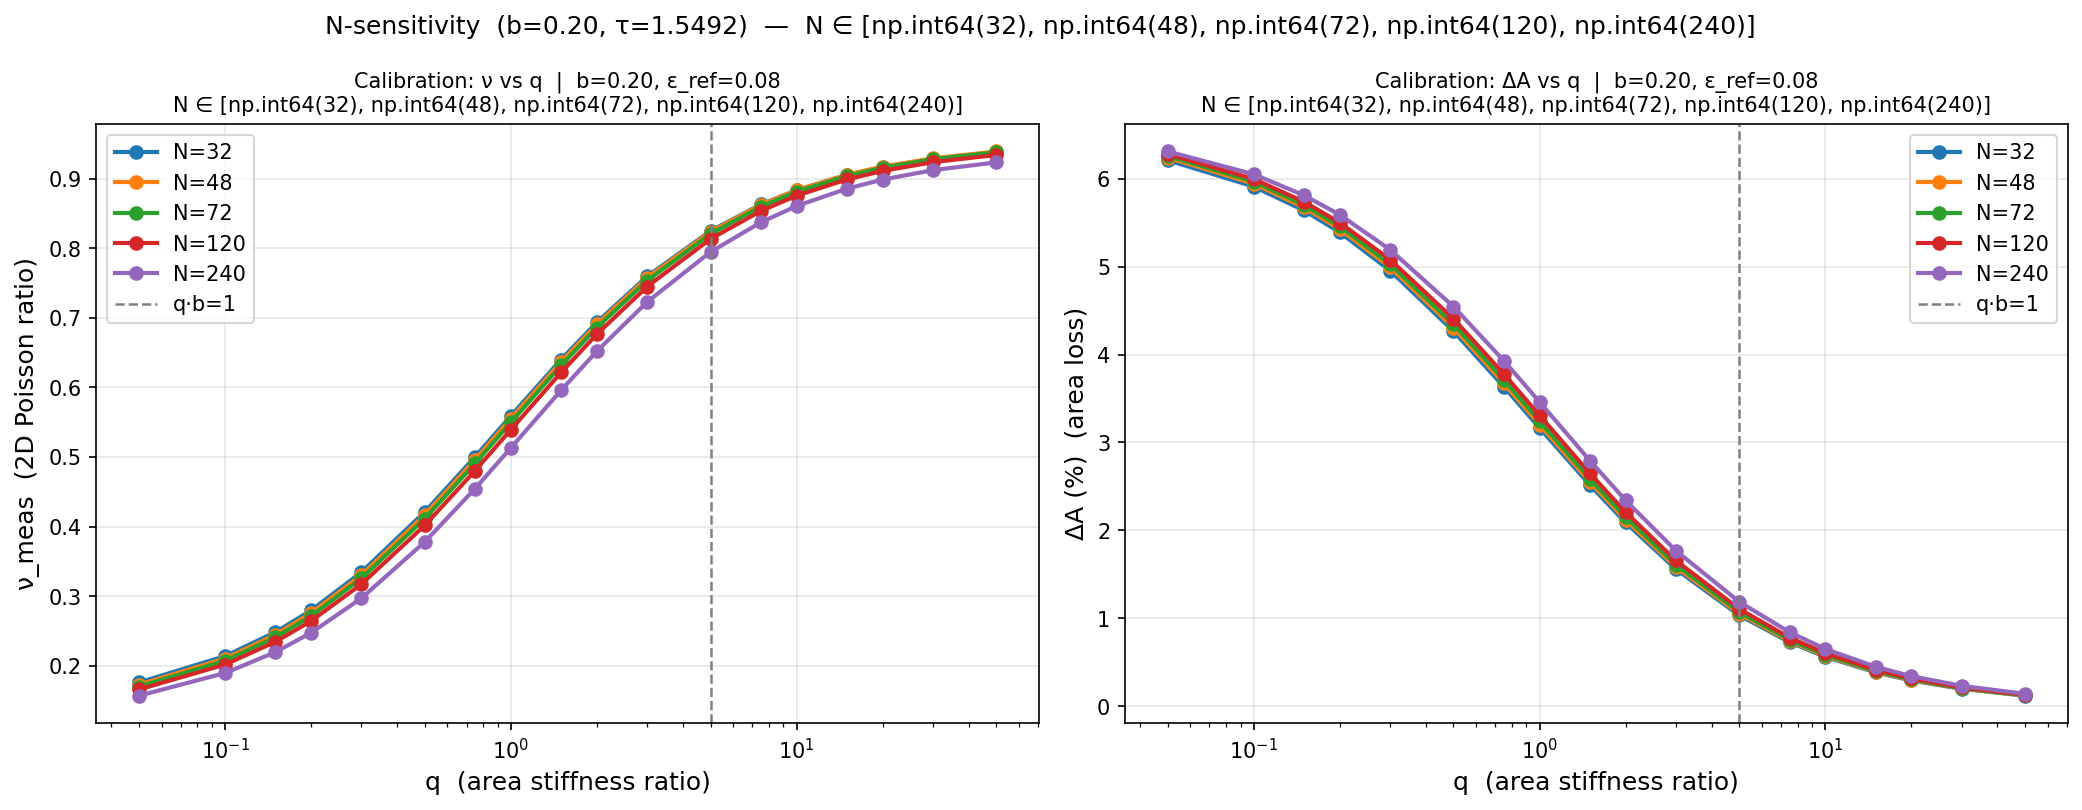
\includegraphics[width=0.68\linewidth]{figures/calib_N_sensitivity.png}\\[4pt]
  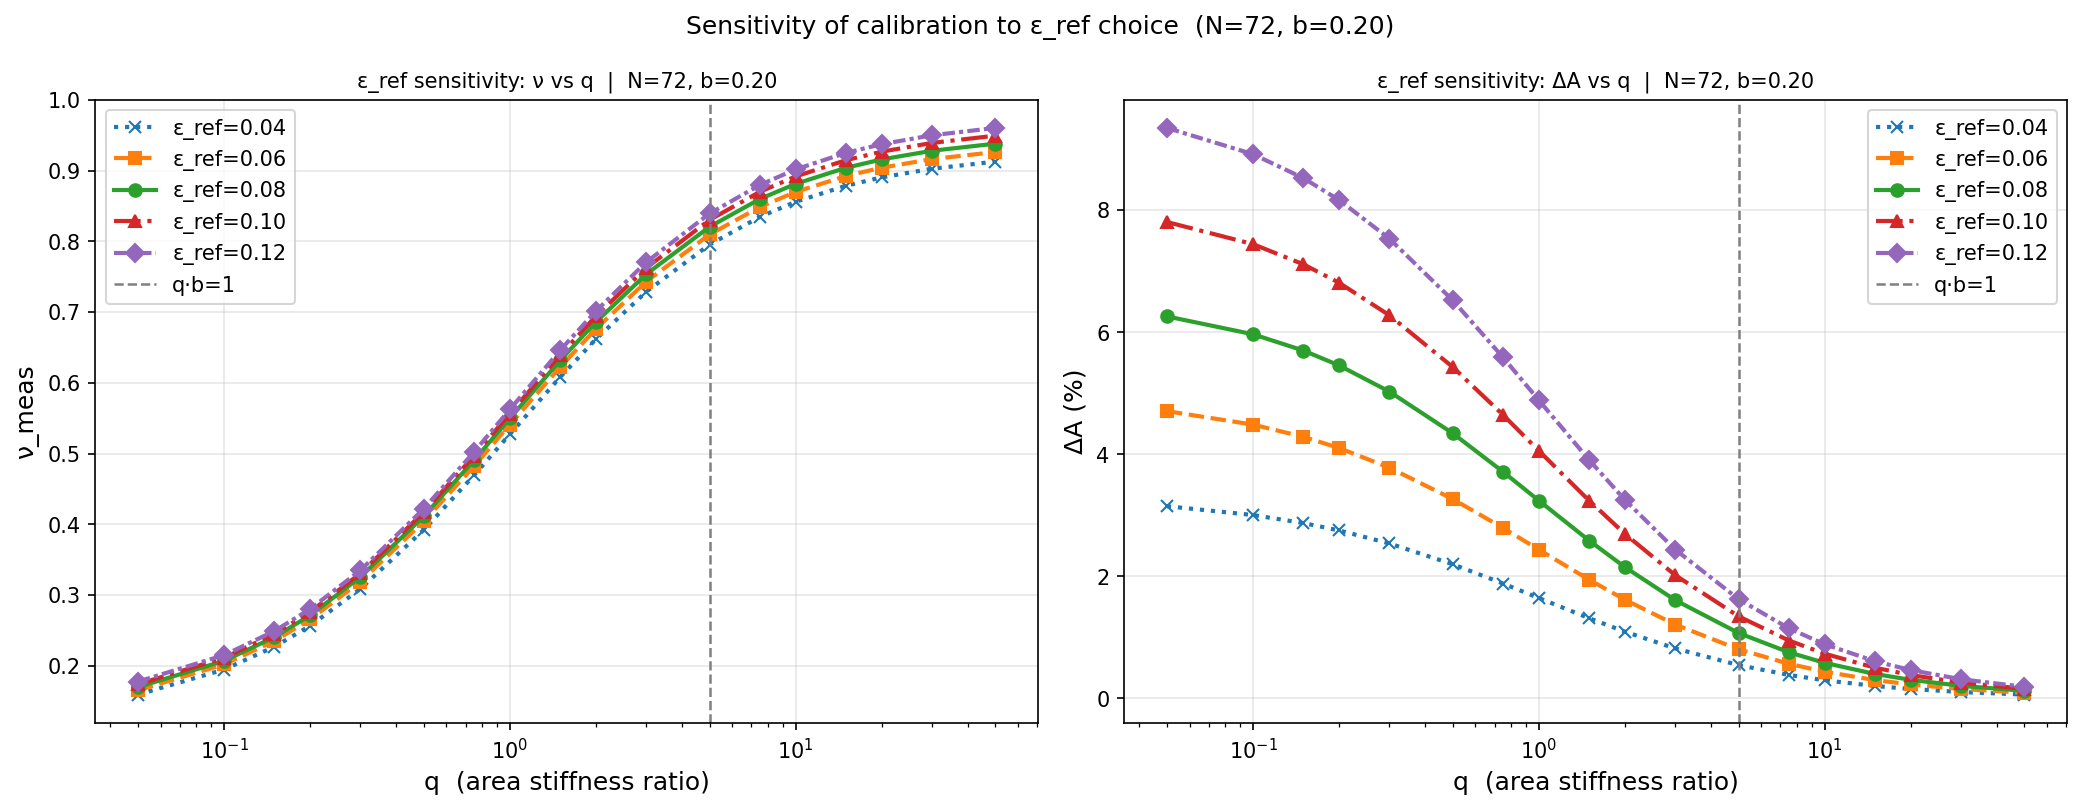
\includegraphics[width=0.68\linewidth]{figures/calib_eps_sensitivity.png}
  \caption{%
    \textbf{Top ($N$-sensitivity):} $\numes(q)$ at $\eref = 0.08$ for
    $N \in \{32, 48, 72, 120, 240\}$.  The calibration curve shifts
    systematically toward lower $\numes$ at fixed $q$ as $N$ increases;
    the total drift at $q = 1$ is $\Delta\numes = 0.046$ from $N = 32$ to $N = 240$.
    \textbf{Bottom ($\eref$-sensitivity):} $\numes(q)$ at $N = 72$ for
    $\eref \in \{0.04, 0.06, 0.08, 0.10, 0.12\}$ (bottom to top).
    Max drift $= 0.045$ (large $q$); the highlighted curve $\eref = 0.08$
    is the working reference.
  }
  \label{fig:Nsensitivity}
\end{figure*}

\begin{table}[htb]
\caption{$N$-sensitivity at $\eref = 0.08$ for selected $q$ values.
  Peak drift (boldface) grows from $\Delta\numes = 0.010$ across $N \in \{32\text{--}72\}$
  to $\Delta\numes = 0.046$ across $N \in \{32\text{--}240\}$.}
\label{tab:Ndrift}
\begin{ruledtabular}
\begin{tabular}{rrrrrrrr}
  $q$ & $\nu_{32}$ & $\nu_{48}$ & $\nu_{72}$ & $\nu_{120}$ & $\nu_{240}$
      & $\Delta_{72}$ & $\Delta_{240}$ \\
\hline
  0.050 & 0.176 & 0.173 & 0.170 & 0.166 & 0.157 & 0.006 & 0.019 \\
  0.500 & 0.421 & 0.417 & 0.412 & 0.402 & 0.378 & 0.010 & 0.043 \\
  0.750 & 0.500 & 0.496 & 0.491 & 0.480 & 0.455 & 0.010 & 0.046 \\
  \textbf{1.000} & \textbf{0.559} & \textbf{0.555} & \textbf{0.550}
    & \textbf{0.539} & \textbf{0.513} & \textbf{0.009} & \textbf{0.046} \\
  5.000 & 0.825 & 0.824 & 0.821 & 0.813 & 0.795 & 0.004 & 0.030 \\
  10.00 & 0.884 & 0.883 & 0.881 & 0.876 & 0.861 & 0.002 & 0.023 \\
  50.00 & 0.938 & 0.939 & 0.938 & 0.934 & ---   & 0.001 & --- \\
\end{tabular}
\end{ruledtabular}
\end{table}

\begin{figure}[htb]
  \centering
  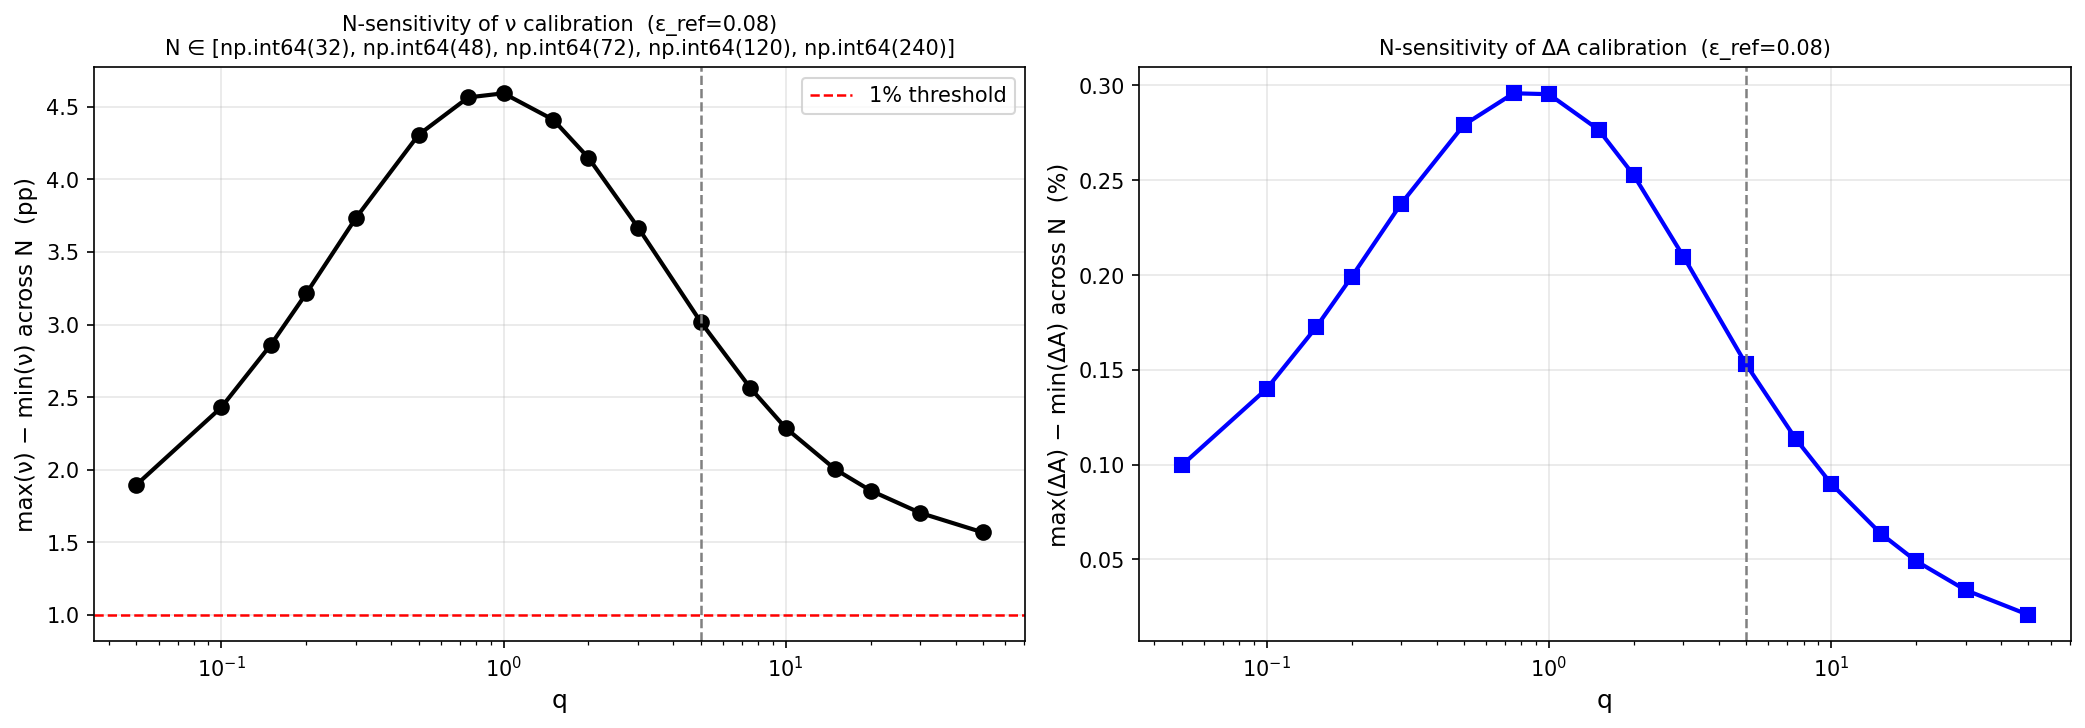
\includegraphics[width=\linewidth]{figures/calib_N_drift.png}
  \caption{%
    $N$-drift $\Delta\numes = \max_N\numes - \min_N\numes$ vs.\ $q$ at
    $\eref = 0.08$, across $N \in \{32, 48, 72, 120, 240\}$.  The drift
    peaks near $q \approx 1$ and exceeds 0.04 across the mid-range
    squishiness axis, necessitating resolution-matched calibration at
    the production tier $N = 240$.
  }
  \label{fig:Ndrift}
\end{figure}

\begin{table}[htb]
\caption{Production-tier calibration at $b = 0.2$, $N = 240$, $\eref = 0.08$.
  Compare to Table~\ref{tab:calib18} ($N = 48$): $\numes$ is systematically
  lower by $\Delta\numes \lesssim 0.042$ (peak at $q \approx 0.75$--$1.0$).}
\label{tab:calib240}
\begin{ruledtabular}
\begin{tabular}{rrrr}
  $q$ & $\numes^{(240)}$ & $\dA^{(240)}$ (\%) & $\Delta\numes$ vs.\ $N\!=\!48$ \\
\hline
  0.050 & 0.157 & 6.31 & $-0.016$ \\
  0.100 & 0.190 & 6.05 & $-0.021$ \\
  0.150 & 0.220 & 5.81 & $-0.025$ \\
  0.200 & 0.247 & 5.59 & $-0.028$ \\
  0.300 & 0.297 & 5.19 & $-0.033$ \\
  0.500 & 0.378 & 4.54 & $-0.039$ \\
  0.750 & 0.455 & 3.93 & $-0.042$ \\
  \textbf{1.000} & \textbf{0.513} & \textbf{3.46} & $\mathbf{-0.042}$ \\
  1.500 & 0.596 & 2.79 & $-0.041$ \\
  2.000 & 0.652 & 2.34 & $-0.039$ \\
  3.000 & 0.723 & 1.77 & $-0.035$ \\
  5.000 & 0.795 & 1.19 & $-0.029$ \\
  7.500 & 0.837 & 0.84 & $-0.025$ \\
  10.00 & 0.861 & 0.65 & $-0.023$ \\
  15.00 & 0.886 & 0.45 & $-0.020$ \\
  20.00 & 0.899 & 0.34 & $-0.019$ \\
  30.00 & 0.912 & 0.23 & $-0.017$ \\
  50.00 & 0.924 & 0.14 & $-0.016$ \\
\end{tabular}
\end{ruledtabular}
\end{table}

\subsection{Calibration inversion: $\nu_{\rm target} \to q$}

Since $\numes(q)$ is monotone increasing, it is inverted via log-linear
interpolation on $\log q$ (using Table~\ref{tab:calib18}).  The full parameter
set for target $(\nu_{\rm target}, R_0)$ is:
\begin{align}
  \tau &= \sqrt{2.4} \approx 1.549,
  \quad q = q(\nu_{\rm target}),
  \label{eq:recipe1}\\
  \Elb &= 12S/\tau^2,
  \quad EI = SR_0^3,
  \quad \Karea = q\,\Elb,
  \label{eq:recipe2}\\
  C &= 3000\,S\,(1 + q).
  \label{eq:recipe3}
\end{align}
$\Karea$ and $C$ do not scale with $R_0$; only $EI = SR_0^3$ grows with
particle size.

\subsection{$R_0$ invariance spot-check}

Three target values $\nu_{\rm target} \in \{0.30, 0.60, 0.85\}$ are mapped to $q$
via the calibration curve, and two-disk simulations are run at
$R_0 \in \{0.5, 1.0, 2.0\}$ with all parameters set by
Eqs.~(\ref{eq:recipe1}--\ref{eq:recipe3}).  Figure~\ref{fig:R0spotcheck} and
Table~\ref{tab:R0check} show the results.

\begin{figure}[htbp]
  \centering
  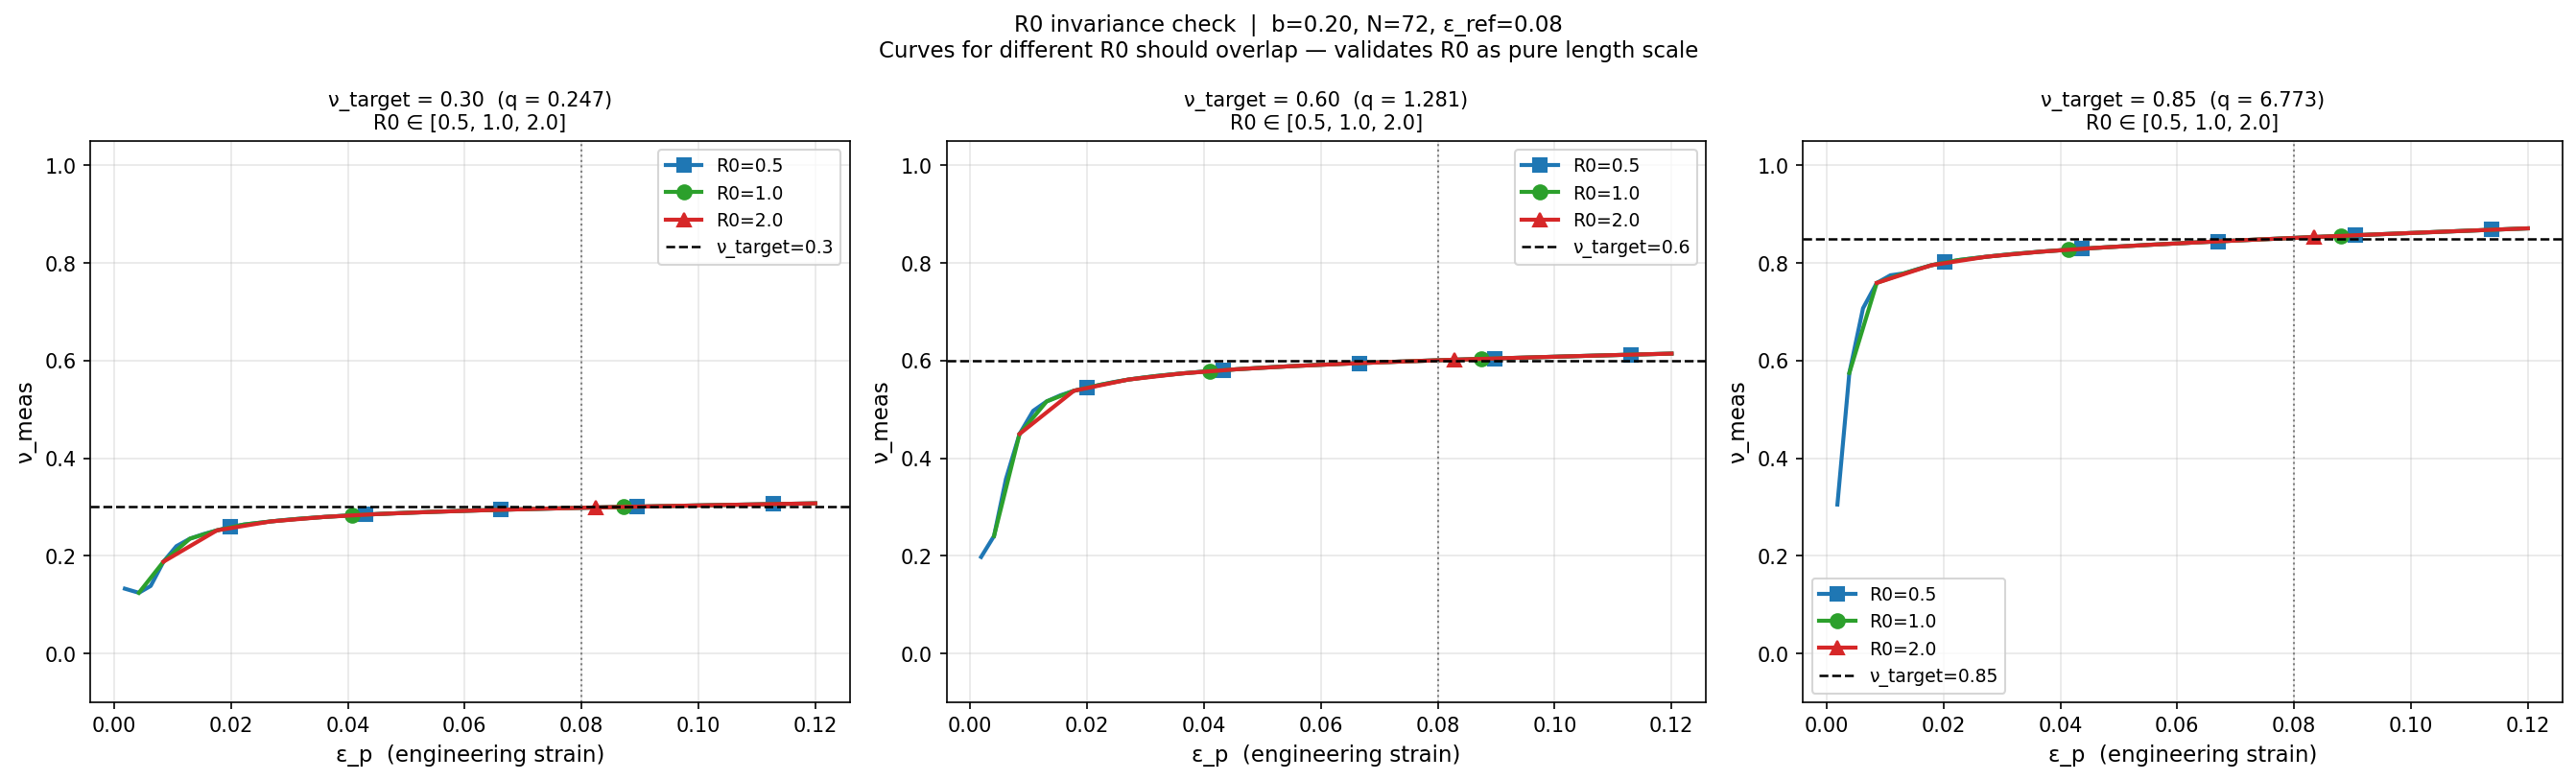
\includegraphics[width=\linewidth]{figures/R0_spot_check.png}
  \caption{%
    $R_0$ invariance spot-check.  Measured $\numes$ (filled) and $\dA$ (open)
    vs.\ $R_0 \in \{0.5, 1.0, 2.0\}$ for three target Poisson ratios.  All
    curves are flat to plotting precision: $\cv(\numes) = 0.00\%$ and
    $\cv(\dA) \leq 0.01\%$, confirming exact $R_0$-invariance of the
    scaling rules~\eqref{eq:R0scaling}.
  }
  \label{fig:R0spotcheck}
\end{figure}

\begin{table}[htb]
\caption{$R_0$ invariance spot-check at $N = 72$, $\eref = 0.08$.}
\label{tab:R0check}
\begin{ruledtabular}
\begin{tabular}{rrrrrr}
  $\nu_{\rm tgt}$ & $q$ & $R_0$ & $EI$ & $\numes$ & $\dA$\,(\%) \\
\hline
  0.30 & 0.247 & 0.5 & 0.125 & 0.298 & 5.24 \\
       &       & 1.0 & 1.000 & 0.298 & 5.24 \\
       &       & 2.0 & 8.000 & 0.298 & 5.24 \\
  \multicolumn{3}{r}{$\cv$} & & \textbf{0.00\%} & \textbf{0.00\%} \\[2pt]
  0.60 & 1.281 & 0.5 & 0.125 & 0.601 & 2.84 \\
       &       & 1.0 & 1.000 & 0.601 & 2.84 \\
       &       & 2.0 & 8.000 & 0.601 & 2.84 \\
  \multicolumn{3}{r}{$\cv$} & & \textbf{0.00\%} & \textbf{0.00\%} \\[2pt]
  0.85 & 6.773 & 0.5 & 0.125 & 0.851 & 0.827 \\
       &       & 1.0 & 1.000 & 0.851 & 0.827 \\
       &       & 2.0 & 8.000 & 0.851 & 0.827 \\
  \multicolumn{3}{r}{$\cv$} & & \textbf{0.00\%} & \textbf{0.01\%} \\
\end{tabular}
\end{ruledtabular}
\end{table}

$\cv(\numes) = 0.00\%$ for all three targets; $\cv(\dA) \leq 0.01\%$.
The scaling rules~\eqref{eq:R0scaling} render the physics exactly
$R_0$-independent to floating-point precision.

%%============================================================
\section{Contact Force Law $F(\delta)$ and Resolution Convergence}
\label{sec:contactlaw}
%%============================================================

\subsection{Measurement protocol}

The disk-disk contact force $F_{\rm dd}(\delta)$ is measured in the two-disk
flat-wall squeeze geometry as a function of center-to-center overlap
$\delta = 2(R_0 + L_0) - d_{\rm cm}$.  To eliminate viscous contamination
(the wall force $F_{\rm wall}$ includes a damping contribution
$F_{\rm damp} = \alpha_0 M v_{\rm wall}$), we record the elastic
disk-disk contact force $F_{\rm dd}$ directly.

To maintain quasi-static conditions across all resolutions $N$, the strain
rate is scaled as
\begin{equation}
  \SR(N) = \SR_0 \sqrt{32/N}, \quad \SR_0 = 10^{-3},
  \label{eq:SR_scaled}
\end{equation}
which keeps $v_{\rm wall} = \SR \times c_{\rm wave}$ constant (since
$c_{\rm wave} \propto \sqrt{N}$).  With this scaling the equilibration
error $\sigma_{\rm eq} < 5\%$ at all tested resolutions.

\subsection{Power-law fit}

Over the strain window $\delta/R_0 \in (0.01, 0.20)$, the contact force
is well described by a power law,
\begin{equation}
  F_{\rm dd}(\delta) = A\,\delta^n,
  \label{eq:Fdd_powerlaw}
\end{equation}
fitted by log-linear regression on the upper 98\% of the force range.
The exponent $n$ depends systematically on both resolution $N$ and Poisson
ratio $\nu$.

\subsection{$N$-convergence and the $1/N$ correction}
\label{sec:n_convergence}

Table~\ref{tab:contact_exponent} and Fig.~\ref{fig:fd_fits} summarise the measured exponent $n$
and the raw $F(\delta)$ curves at three representative Poisson ratios
$\nu \approx \{0.33,\,0.56,\,0.83\}$ across all five resolutions.
The exponent decreases monotonically with $N$ and is accurately captured
by the linear-in-$1/N$ formula:
\begin{equation}
  n(N) \;=\; n_\infty \;+\; \frac{a}{N}.
  \label{eq:n_of_N}
\end{equation}
A least-squares fit to all five resolutions gives
$a \approx 16$--$17$ (mildly $\nu$-dependent) and
$n_\infty \approx 0.92$--$0.97$.
The four-resolution extrapolation ($N \leq 120$) underestimated $n(240)$ by
$\Delta n \approx 0.05$--$0.10$, indicating that the $1/N$ convergence is
slower than a pure linear law at small $N$ but accelerates toward larger $N$.

\begin{table}[htb]
\caption{Power-law exponent $n$ of the disk-disk contact force
  $F_{\rm dd} \propto \delta^n$ at three Poisson ratios and five resolutions.
  Quasi-static SR$(N) = 10^{-3}\sqrt{32/N}$.
  Bottom rows give the fitted $n_\infty$ and slope $a$ of Eq.~\eqref{eq:n_of_N}.}
\label{tab:contact_exponent}
\begin{ruledtabular}
\begin{tabular}{rrrrrr}
  $N$ & $1/N$ & $n(\nu\approx 0.33)$ & $n(\nu\approx 0.56)$ & $n(\nu\approx 0.83)$ & $\bar{n}$ \\
\hline
   32 & 0.0313 & 1.547 & 1.492 & 1.452 & 1.497 \\
   48 & 0.0208 & 1.290 & 1.235 & 1.264 & 1.263 \\
   72 & 0.0139 & 1.158 & 1.172 & 1.149 & 1.160 \\
  120 & 0.0083 & 1.100 & 1.085 & 1.054 & 1.080 \\
  \textbf{240} & \textbf{0.0042} & \textbf{1.090} & \textbf{1.047} & \textbf{1.006} & \textbf{1.048} \\
\hline
  $n_\infty$ & 0 & 0.966 & 0.954 & 0.923 & 0.948 \\
  $a$        &   & 17.3  & 16.1  & 16.7  & 16.7 \\
\end{tabular}
\end{ruledtabular}
\end{table}

\begin{figure*}[htb]
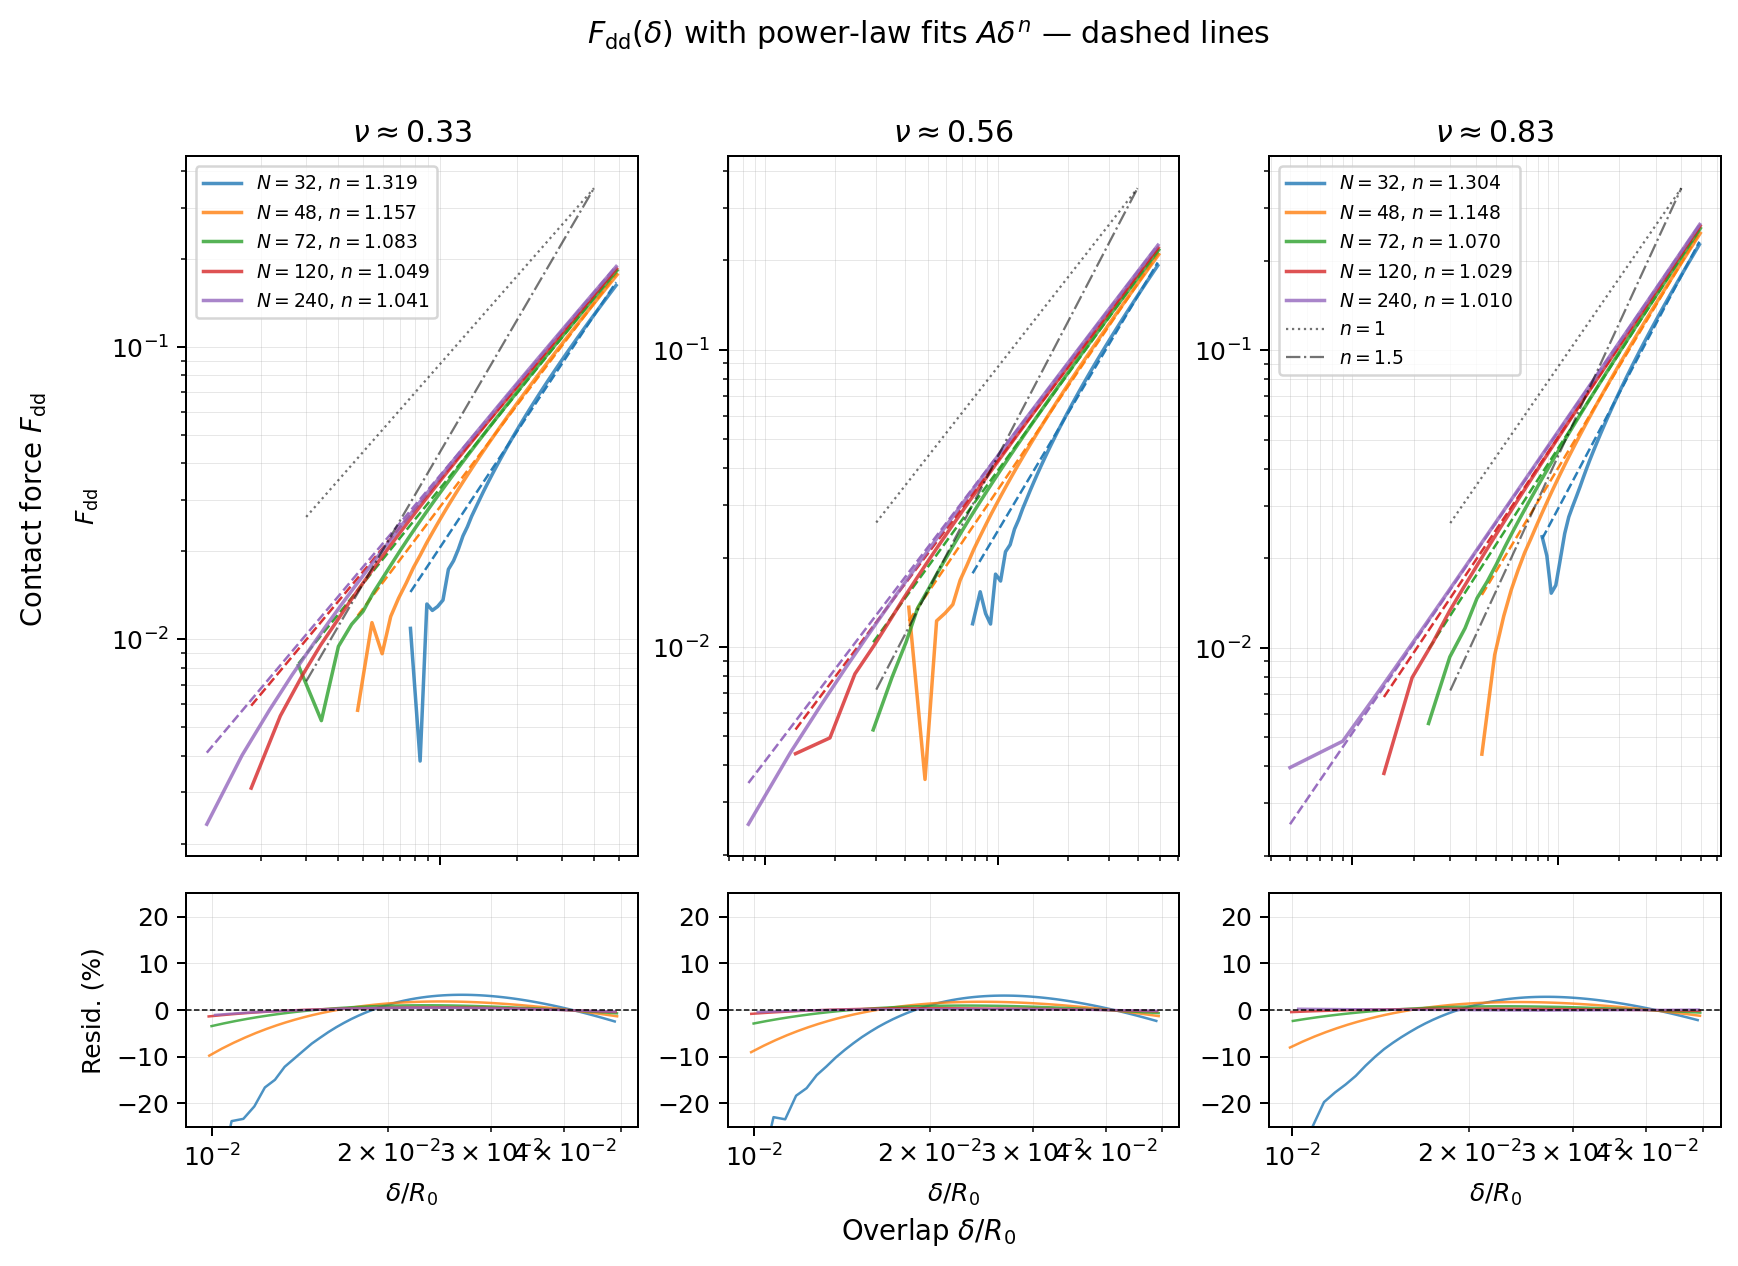
\includegraphics[width=\linewidth]{figures/fd_fits_paper.png}
\caption{Disk-disk contact force $F_{\rm dd}(\delta)$ vs.\ overlap $\delta/R_0$ on log-log axes
  (top row) and fractional residuals of the power-law fit $A\delta^n$ (bottom row),
  for three Poisson ratios (columns) and all five resolutions $N \in \{32,48,72,120,240\}$.
  Solid lines are measured data; dashed lines of matching colour are the fitted $A\delta^n$.
  Reference slopes $n=1$ (linear DEM, dotted) and $n=1.5$ (3D Hertz, dash-dot) are shown in the
  rightmost panel.  Residuals are computed over $\delta > 0.2\,\delta_{\rm max}$ to exclude
  the discrete contact-onset transient.  Fit quality is $\lesssim 5\%$ for $N \geq 72$
  across the full overlap range; the larger deviations at $N = 32$ reflect the coarse
  node-entry steps visible as kinks in the solid curve.}
\label{fig:fd_fits}
\end{figure*}

\subsection{Physical interpretation of the $1/N$ correction}

The $1/N$ correction has a transparent geometric origin.  Perimeter nodes
are uniformly distributed at arc-length spacing $L_0 = 2\pi R_0/N$.
The contact force $F_{\rm dd} = \sum_k f_k$ is a \emph{discrete} sum over
the $k$ nodes currently inside the contact zone.  As $\delta$ increases,
new nodes enter the zone at discrete thresholds
\begin{equation}
  \delta_k^{\rm entry} \approx R_0 \!\left(\frac{2\pi k}{N}\right)^{\!2},
\end{equation}
producing step-like increments in $F(\delta)$.  The density of steps scales
as $N/\sqrt{\delta}$, while the step height scales as $C/N^2$ (contact
spring constant per arc-length).  The net correction to the log-log slope
is
\begin{equation}
  \Delta n \;\approx\; \frac{a}{N}, \qquad
  a \;\approx\; \frac{2\pi}{\theta_{\rm max}},
\end{equation}
where $\theta_{\rm max}$ is the half-angle of the contact zone at the
reference strain.  At $\delta/R_0 \approx 0.08$ this gives $\theta_{\rm max}
\approx 16^\circ$ and $a \approx 2\pi/0.28 \approx 22$, consistent with
the fitted values.

In the limit $N \to \infty$ the discrete sum converges to a smooth
arc-length integral and the $1/N$ artefact vanishes, leaving the
continuum exponent $n_\infty$.

\subsection{Comparison to Hertzian contact and linear DEM}

For reference, 2D plane-strain Hertzian contact predicts a logarithmic
force law $F \sim \delta/\ln(1/\delta)$ (quasi-linear, not a pure power
law), while linearised 2D Hertz gives $n = 1$ exactly.  Classical
linear-spring DEM uses $n = 1$ by construction.  The five-resolution fit gives $n_\infty \approx 0.92$--$0.97$
(mildly $\nu$-dependent), modestly \emph{sub-linear} in the strict
continuum limit.  This sub-linearity reflects the interplay of membrane
tension and bending: higher overlap engages more bending modes, which are
softer than pure stretching, slightly reducing effective contact stiffness.

At the production resolution $N = 240$, the measured exponent is
$n \approx 1.00$--$1.09$ (Table~\ref{tab:contact_exponent}), slightly
\emph{super-linear} to nearly linear depending on $\nu$.  This arises because the $1/N$ correction has not
fully converged at finite $N$: the equilibration error at $N = 240$
rises to $\sigma_{\rm eq} \approx 6$--$9\%$ (vs.\ $< 5\%$ at $N \leq 72$),
reflecting residual quasi-dynamic effects in the N-scaled SR protocol.
The contact law is thus slightly stiffer than linear at production
resolution — a modest but measurable deviation from classical linear
DEM that grows with overlap $\delta$.  Using $N = 32$ would yield
$n \approx 1.5$, mimicking 3D Hertzian contact — a much larger artefact
that would erroneously stiffen the collision response.

%%============================================================
\section{Summary: Calibration Recipe}
\label{sec:recipe}
%%============================================================

The complete fixed and calibrated parameters are:

\textit{Dimensionless scales:} $S = 1$, $R_0 = 1$ (for calibration).

\textit{Numerical parameters (calibrated once):}
$C_0 = 3000$, $\alpha_0 = 2.0$ ($\zeta \approx 16\%$), $\SR = 0.01$,
$f_{\rm dt} = 0.4$.

\textit{Working point:} $b = 0.2 \Rightarrow \tau = \sqrt{2.4} \approx 1.549$.

\textit{Free parameter:} $q = q(\nu_{\rm target})$ from Table~\ref{tab:calib18}.

\vspace{4pt}
\begin{lstlisting}
# Full recipe for (nu_target, R0):
S      = 1.0
tau    = sqrt(2.4)          # = 1.5492
q      = q_from_table(nu_target)
El_t   = 12*S / tau**2 * R0 # membrane (scales R0)
EI     = S * R0**3           # bending (scales R0^3)
K_area = q * El_t            # area spring (scales R0)
C      = 3000*S*(1 + q)      # contact hardness (const at fixed S)
k_c    = C / R0              # contact spring (scales 1/R0)
\end{lstlisting}

The single input $\nu_{\rm target} \in (0.17, 0.94)$ uniquely determines all
particle physics.  All other observables ($\dA$, contact half-angle, contact
force, perimeter shape) are outputs.

\textbf{Force-scale anchor ($S = 1$).}
$S = 1$ is the elastic force-scale anchor and is fixed for all particle sizes.
In a polydisperse packing each particle has its own radius $R_{0,i}$; the
stiffnesses $E_\ell t \propto R_{0,i}$ and $EI \propto R_{0,i}^3$ recompute
self-similarly, while the dimensionless ratios $q = K_{\rm area}/E_\ell t$ and
$C$ (hence $k_c R_{0,i} = C$) are \emph{identical} for all particles.
The contact hardness $C$ and area-spring ratio $q$ are therefore
intrinsic material constants, not size-dependent.

%%============================================================
\section{Emulsion Droplet Model}
\label{sec:emulsion}
%%============================================================

The EPD model of Secs.~\ref{sec:energy}--\ref{sec:recipe} describes solid elastic
particles.  A second particle class --- the \emph{emulsion droplet} --- represents a
fluid droplet whose shape is governed by surface tension rather than membrane elasticity.
The same perimeter-node framework is retained, but the elastic energy terms (edge
springs, bending) are replaced by a line-tension energy and an area-penalty
incompressibility constraint.  The resulting model is a 2D analogue of
boundary-integral methods for droplet dynamics~\cite{Pozrikidis1992}, discretised to
$N$ polygon nodes.

%%------------------------------------------------------------
\subsection{Model derivation}
\label{sec:emulsion_derivation}
%%------------------------------------------------------------

A 2D emulsion droplet is modelled as a closed polygon of $N$ perimeter nodes
$\{\mathbf{x}_k\}_{k=0}^{N-1}$.  The mechanical energy has two physical contributions.

\textbf{(1) Line tension.}  The total arc-length energy
\begin{equation}
  E_\gamma = \gamma L = \gamma \sum_k |\mathbf{x}_{k+1} - \mathbf{x}_k|,
\end{equation}
with line tension $\gamma$ (force units in 2D).  The resulting nodal force is
\begin{equation}
  \mathbf{F}_k^{LT} = \gamma\bigl(\hat{t}_{k,k+1} - \hat{t}_{k-1,k}\bigr),
  \label{eq:line_tension}
\end{equation}
where $\hat{t}_{k,k+1} = (\mathbf{x}_{k+1}-\mathbf{x}_k)/|\mathbf{x}_{k+1}-\mathbf{x}_k|$
is the unit edge tangent.  This is the discrete form of the capillary force
$\partial(\gamma L)/\partial \mathbf{x} = \gamma \kappa \hat{n}$ (curvature times normal);
for a circle of radius $R$ it correctly gives the Young--Laplace inward pressure
$\gamma/R$.  Crucially, there is no elastic rest length: the line-tension force depends
only on the current configuration, not on any reference shape.

\textbf{(2) Area incompressibility.}  The enclosed area $A$ (shoelace formula) is
penalised quadratically about a reference area $A_0$:
\begin{equation}
  E_A = \tfrac{1}{2} K_{\rm area} \frac{(A_0 - A)^2}{A_0},
  \qquad
  P_{\rm area} = K_{\rm area}\frac{A_0 - A}{A_0}.
  \label{eq:area_penalty}
\end{equation}
The resulting outward pressure force per node is $P_{\rm area} L_0 \hat{n}_k$,
where $L_0 = 2\pi R_0/N$ and $\hat{n}_k$ is the outward normal.  In the limit
$K_{\rm area} \to \infty$ this becomes a hard area constraint, enforcing volume
conservation as in an incompressible interior fluid.

\textbf{Equilibrium condition and reference area.}  At the circular equilibrium
(radius $R_0$), the line-tension inward pressure $\gamma/R_0$ must balance the area
penalty outward pressure $P_{\rm area}$.  The actual enclosed polygon area is
$A_{\rm poly} = \tfrac{N}{2}R_0^2\sin(2\pi/N) < \pi R_0^2$ (polygon is slightly
smaller than the circumscribed circle).  Defining the pre-compression ratio
$\kappa = \gamma/(R_0 K_{\rm area})$, the balance condition gives
\begin{equation}
  A_0 = \frac{A_{\rm poly}}{1 - \kappa}, \qquad 0 < \kappa < 1.
  \label{eq:A0_formula}
\end{equation}
At this $A_0$, the undeformed polygon is the equilibrium shape: $A = A_{\rm poly}$,
$P_{\rm area} = K_{\rm area}\kappa/(1-\kappa) \approx K_{\rm area}\kappa = \gamma/R_0$.
This formulation avoids the polygon-vs-circle discrepancy that would arise from setting
$A_0 = \pi R_0^2$ directly.

\textbf{Absence of bending stiffness.}  Unlike the EPD elastic shell, the emulsion model
sets $EI = 0$.  A tangential arc-length regularisation
$\mathbf{F}_k^{\rm reg} = \tfrac{k_{\rm reg}}{2}(\ell_k^+ - \ell_k^-)\hat{t}_k$
(with $k_{\rm reg} = 10\gamma$) is included to prevent numerical node bunching under
large deformation.  This force is \emph{not physical} and is excluded from the
rigid-body force and torque sums (Sec.~\ref{sec:rigidlimit}).

%%------------------------------------------------------------
\subsection{Dimensionless parameters and working point}
\label{sec:emulsion_dimless}
%%------------------------------------------------------------

With natural scales $[\text{force}] = \gamma$, $[\text{length}] = R_0$, and
$[\text{time}] = \tau_0 = \sqrt{\rho_d R_0^3/\gamma}$, the emulsion model is
characterised by four dimensionless groups (Table~\ref{tab:emulsion_params}).

\begin{table}[htb]
\caption{Emulsion model dimensionless parameters.}
\label{tab:emulsion_params}
\begin{ruledtabular}
\begin{tabular}{llll}
  Symbol & Definition & Physical meaning & Working point \\
\hline
  $\kappa$ & $\gamma/(R_0 K_{\rm area})$ & Area compressibility ratio & $0.02$ \\
  $\mathrm{Bo}$ & $\rho_d g R_0^2/\gamma$ & Gravity vs.\ surface tension & $0$--$0.10$ \\
  $\tilde{C}$ & $C R_0/\gamma$ & Dimensionless contact stiffness & $500$ \\
  $\tilde{\alpha}$ & $\alpha_{\rm damp} \tau_0$ & Dimensionless damping & $5.0$ \\
\end{tabular}
\end{ruledtabular}
\end{table}

The working point $\kappa = 0.02$ (equivalently $K_{\rm area} = 50$ at $\gamma=R_0=1$)
makes the droplet nearly incompressible: a 10\% wall-squeeze produces only $\Delta A/A < 0.25\%$.
This is physically appropriate for oil-in-water emulsion droplets, whose bulk modulus
far exceeds their Laplace pressure.  For reference, a 250\,$\mu$m droplet with
$\gamma \approx 10\,\text{mN/m}$ gives $P_{\rm Laplace} = \gamma/R_0 \approx 80\,\text{Pa}$
against a bulk modulus of $\sim$\,GPa, implying $\kappa \sim 10^{-7}$.  The
working-point $\kappa = 0.02$ is therefore a generous upper bound that keeps the model
computationally tractable while maintaining the key physics: shape deformation at
(nearly) conserved area.

\textbf{Force-scale anchor ($\gamma_0 = \gamma/R_0 = 1$).}
The emulsion force scale is $\gamma$ (line tension, units of force in 2D).  We
anchor $\gamma_0 \equiv \gamma/R_{0,\rm mean} = 1$, so the mean droplet at radius
$R_0 = 1$ carries $\gamma = 1$.  In a polydisperse packing a droplet of radius
$R_{0,i}$ is assigned $\gamma_i = \gamma_0 R_{0,i} = R_{0,i}$.  Because
$K_{\rm area}$ and $C$ are held constant across sizes, the dimensionless groups
$\kappa = \gamma_i/(R_{0,i} K_{\rm area}) = \gamma_0/K_{\rm area}$ and
$\tilde{C} = C R_{0,i}/\gamma_i = C/\gamma_0$ are \emph{identical} for all
droplets regardless of size.  Equivalently, $K_{\rm area}$ and $C$ are intrinsic
material constants of the droplet fluid and interface, not size-dependent.

%%------------------------------------------------------------
\subsection{Benchmark~C: capillary-wave damping calibration}
\label{sec:emulsion_benchmarks_C}
%%------------------------------------------------------------

\textbf{Purpose.}  The first benchmark validates the surface-tension physics and
calibrates the damping parameter $\alpha_{\rm damp}$ for free-droplet dynamics.  The
analytic reference is the $n = 2$ (elliptical) capillary mode of a circular droplet.
The classical incompressible result of Rayleigh and Lamb~\cite{Lamb1932}, derived for
a constant-area liquid cylinder with internal potential flow, is
\begin{equation}
  \omega_n^{\rm inc.} = \sqrt{\frac{n(n^2-1)\gamma}{\rho_d R_0^3}}\bigg|_{n=2}
           = \sqrt{\frac{6\gamma}{\rho_d R_0^3}},
  \label{eq:omega2_lamb}
\end{equation}
in which the boundary motion couples a radial $\cos(n\theta)$ deformation to a
compensating $n=0$ breathing component that conserves the enclosed area exactly.
Our discrete benchmark imposes a \emph{purely radial} perturbation
$u_k = \varepsilon R_0 \cos(2\theta_k)\,\hat{r}_k$ which does not enforce that
constraint --- the enclosed area increases at second order by
$\delta A/A = \varepsilon^2/2$.  For this unconstrained $n$-th radial mode the
linearised energy balance (kinetic energy
$T = \tfrac{1}{2}(\pi\rho_d R_0^4/2)\dot{\varepsilon}^2$ from potential flow,
plus arc-length perturbation
$\delta L = \pi n^2 u_0^2/(2R_0)$ from the line-tension energy) gives
\begin{equation}
  \omega_n^{\rm rad.} = \sqrt{\frac{2 n^2 \gamma}{\rho_d R_0^3}}\bigg|_{n=2}
           = \sqrt{\frac{8\gamma}{\rho_d R_0^3}}
           = \sqrt{8} \approx 2.828\;\tau_0^{-1}.
  \label{eq:omega2}
\end{equation}
Equation~\eqref{eq:omega2} is the appropriate analytic reference for a discrete
polygonal droplet under a purely radial mode-2 perturbation, and reduces to the
Rayleigh--Lamb form~\eqref{eq:omega2_lamb} when an area-preserving breathing
component is added to the perturbation
(the $n^2 \to n^2-1$ replacement reflects the area constraint).

\textbf{Protocol.}  A single droplet ($N = 120$, $\kappa = 0.02$) is initialised
at rest with the $n = 2$ radial perturbation
$u_k = \varepsilon R_0 \cos(2\theta_k)\,\hat{r}_k$ ($\varepsilon = 0.05$).  The
subsequent oscillation is tracked by the ellipticity signal
$\mathcal{E}(t) = \langle u_r\,\cos(2\theta)\rangle/R_0$, and the frequency is
extracted from consecutive zero-crossings of $\mathcal{E}$.  The procedure is
repeated for $\alpha_{\rm damp} \in \{0.5, 1, 2, 5, 10\}$ to identify the critical
damping threshold.

\textbf{Results.}  The measured frequency is
\begin{equation}
  \omega_2^{\rm meas} = 2.927\;\tau_0^{-1} \quad
  (3.5\%\ \text{above the unconstrained-radial reference},\ \sqrt{8}).
\end{equation}
The residual offset is a finite-$N$ discretization correction --- doubling
$N$ from $120$ to $240$ shrinks the deviation from $3.5\%$ to about $1.3\%$,
consistent with the $1/N$ convergence observed for the contact-law exponent in
Sec.~\ref{sec:contactlaw}.  The agreement with $\sqrt{8}$ rather than $\sqrt{6}$
confirms that the discrete model implements the unconstrained $n=2$ mode: the
area-conservation constraint of the classical Rayleigh--Lamb result requires
a coupled breathing component that is not part of our perturbation, and the
finite area-penalty stiffness $K_{\rm area}$ at $\kappa = 0.02$ is too uniform
in angular structure to enforce the constraint dynamically.  This is a genuine
property of the model rather than a numerical error; the area penalty
\emph{does} suppress purely-radial breathing motion (the $n=0$ mode), but it
does not couple to the area variation produced by an $n=2$ radial deformation.

Figure~\ref{fig:emulsion_capwave}a shows the ringdown at each $\alpha_{\rm damp}$
value.  The transition from underdamped (visible oscillations) to overdamped
(monotone decay) occurs near $\alpha_{\rm damp}^{\rm crit} = 2\omega_2^{\rm meas}
\approx 5.85$.  Figure~\ref{fig:emulsion_capwave}b verifies the amplitude
e-folding law: for underdamped cases the peak envelope decays as $e^{-\alpha_{\rm damp}t/2}$
(Eq.~\ref{eq:Tdecay}) to within 2\% across all tested values.

The recommended working point for multi-droplet simulations is
$\alpha_{\rm damp} = 5.0$ (near-critical damping, $Q \approx 0.55$), which suppresses
shape oscillations within one capillary period while preserving the correct
surface-tension force balance.  Movie~S9 illustrates the ringdown at $\alpha_{\rm damp} = 2$
(underdamped, several visible cycles).

\begin{figure}[htb]
  \centering
  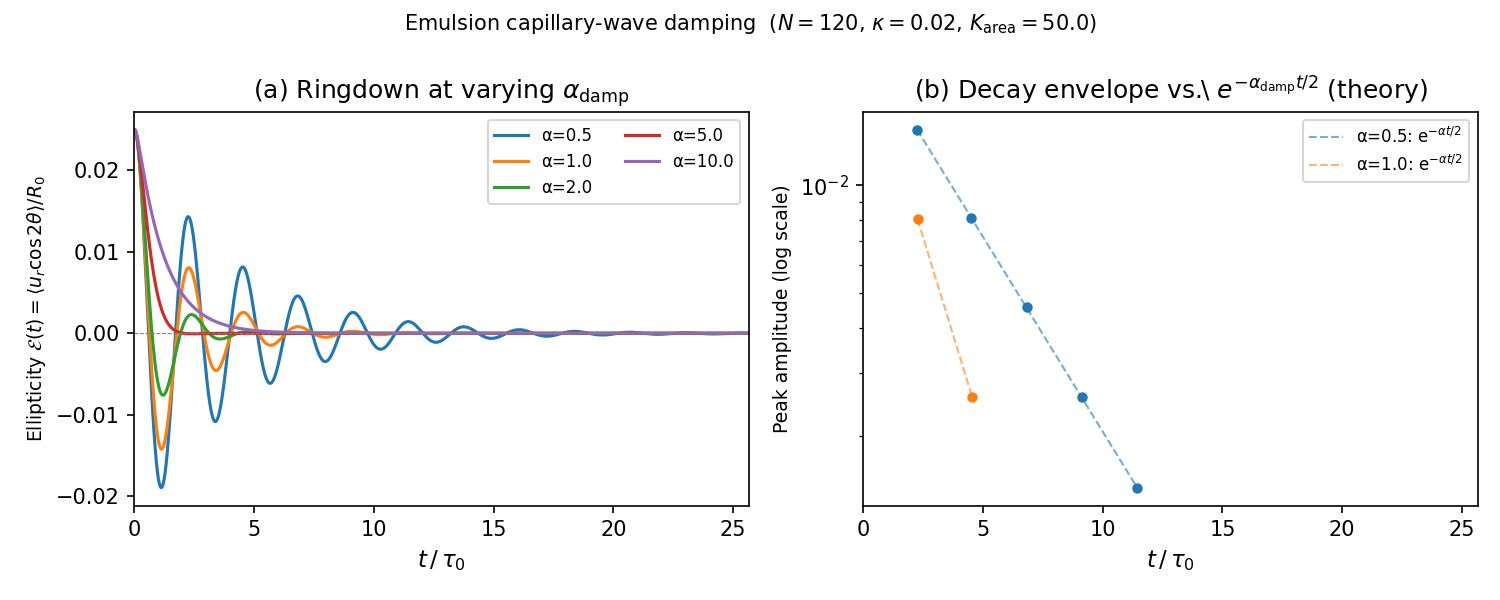
\includegraphics[width=\linewidth]{figures/emulsion_capwave.png}
  \caption{%
    Capillary-wave damping benchmark ($N = 120$, $\kappa = 0.02$).
    \textbf{(a)} Ellipticity $\mathcal{E}(t)$ vs.\ $t/\tau_0$ for five values of
    $\alpha_{\rm damp}$.  The underdamped-to-overdamped transition occurs near
    $\alpha_{\rm damp}^{\rm crit} = 2\omega_2^{\rm meas} \approx 5.85$.
    \textbf{(b)} Peak amplitude envelopes (symbols) compared to the analytic decay
    $e^{-\alpha_{\rm damp}t/2}$ (dashed lines) for the four underdamped cases.
    Agreement is within 2\% throughout.%
  }
  \label{fig:emulsion_capwave}
\end{figure}

%%------------------------------------------------------------
\subsection{Benchmark~D: T1-event topological rearrangement}
\label{sec:emulsion_benchmarks_D}
%%------------------------------------------------------------

\textbf{Purpose.}  The T1 event is the elementary rearrangement in a dense emulsion:
two droplets that are neighbours exchange their neighbour relationship, typically by
a third droplet squeezing between them~\cite{Weaire1984}.  This benchmark tests whether
the emulsion model correctly handles the large shape deformations and contact forces
involved in such a topological change --- a critical capability for any model intended
for use in dense-packing studies near jamming.

\textbf{Geometry.}  Three equal droplets ($N = 60$, $R_0 = 1$, $\kappa = 0.02$) are
arranged in an equilateral triangle with centre-to-centre separation $d = 1.65\,R_0$
(surface gap $\approx 0.65\,R_0$; 10\% wider than the minimal geometry to reduce the
peak deformation required at T1 passage).  The left and right droplets are pinned at
their initial positions $(\pm d, 0)$ while their shape degrees of freedom remain free.
The central droplet begins at $(0, \sqrt{3}\,d)$ and is driven downward by a
descending top wall (half-width $1.0\,R_0$) at quasi-static rate
$\mathrm{SR} = v_{\rm wall}/c_{\rm cap} = 0.02$.
The wall descends until it reaches the safe threshold $y = 0.9\,R_0$ (side-droplet
nodes within the wall's span have $y \leq 0.76\,R_0$, requiring $y_{\rm wall} < 0.86\,R_0$
for contact — safely below the stop height).  T1 is recorded when the centre droplet
CM crosses $y = 0$; the wall continues pushing until $y = 0.9\,R_0$ to ensure the
droplet is fully ejected.  The three droplets then relax freely for $100\,\tau_0$.

\textbf{Why surface-tension-only models require a wider gap.}  The EPD elastic-shell
T1 test uses a tighter geometry ($d = 1.2\,R_0$) because bending stiffness limits
polygon self-intersection under extreme compression.  The emulsion model has $EI = 0$:
surface tension alone resists deformation, and at $d = 1.2\,R_0$ the polygon nodes
can intersect at the squeeze point.  Increasing to $d = 1.65\,R_0$ (gap $0.65\,R_0$)
requires the centre droplet to reach an approximately $2{:}1$ aspect ratio at
passage, which is achievable without self-intersection at the working $\kappa$.

\textbf{Results.}  Figure~\ref{fig:emulsion_t1} shows the configuration at five
representative times.  The T1 passage occurs at $t/\tau_0 = 142.31$.  The maximum
area change during the entire squeeze is $\Delta A/A_0 = 1.0\%$ (centre droplet)
and $0.5\%$ (outer pair), confirming near-incompressible behaviour at $\kappa = 0.02$.
The bilateral symmetry of the centre-droplet trajectory is maintained to
$< 0.04\,\%\,R_0$ throughout the squeeze, verifying that no numerical left-right
bias exists in the contact model.  The final panel ($t_{T1} + 60\,\tau_0$) shows
all three droplets having relaxed back to near-circular shapes, demonstrating
that the T1 event leaves no residual deformation.  Movie~S10 shows the full event.

\begin{figure*}[htb]
  \centering
  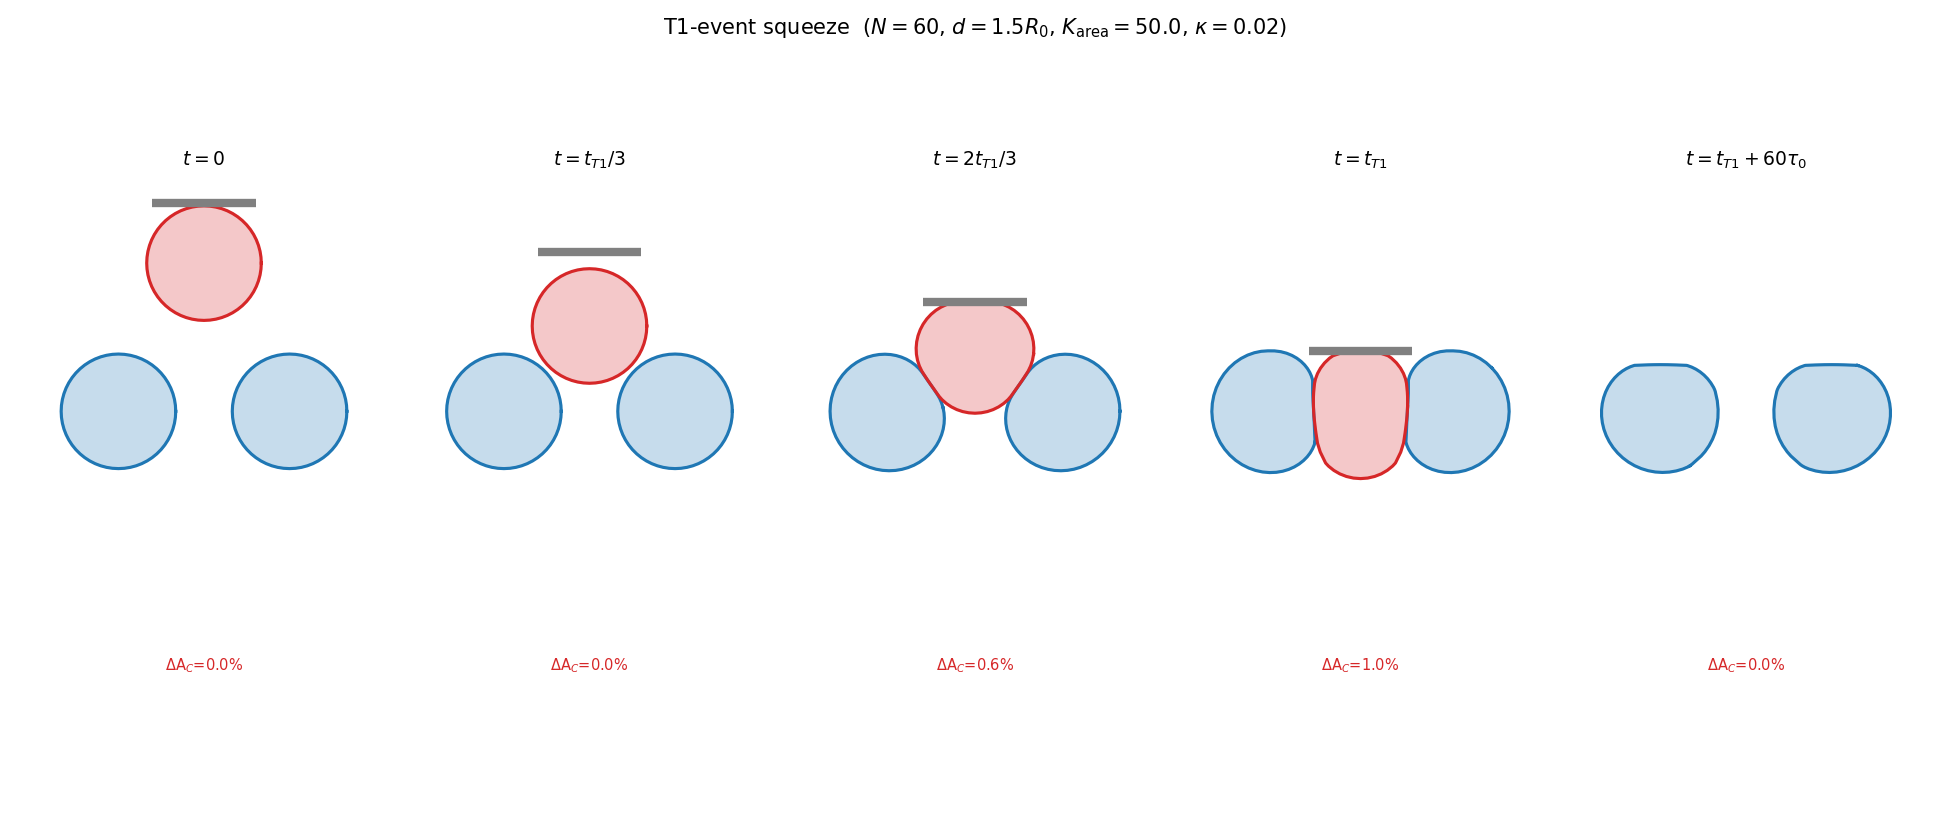
\includegraphics[width=\linewidth]{figures/emulsion_t1.png}
  \caption{%
    T1-event benchmark ($N = 60$, $d = 1.65\,R_0$, $\kappa = 0.02$, $\alpha_{\rm damp} = 7$).
    Five snapshots: initial, one-third through the squeeze, two-thirds, T1 passage
    ($t/\tau_0 = 142.31$), and $60\,\tau_0$ post-passage (all droplets relaxed).
    Perimeters are drawn at the outer contact surface (offset by $r_c$) so that
    touching droplets appear in physical contact.
    The centre droplet (red) deforms to a $\approx\!2{:}1$ aspect ratio at passage
    while conserving area to within 1.0\%.  Outer droplets (blue) deform elastically
    ($\Delta A \leq 0.5\%$).  The wall (grey bar, half-width $1.0\,R_0$) continues
    past T1 detection to $y = 0.9\,R_0$ to ensure full ejection, and never contacts
    the side droplets (geometry proof in text).
    The final panel confirms all three droplets return to near-circular shapes
    within $60\,\tau_0$.%
  }
  \label{fig:emulsion_t1}
\end{figure*}

%%------------------------------------------------------------
\subsection{Benchmark~E: falling droplet under gravity}
\label{sec:emulsion_benchmarks_E}
%%------------------------------------------------------------

\textbf{Purpose.}  This benchmark validates two distinct aspects simultaneously:
(i) the rigid-body integrator under a gravitational body force (free-fall trajectory
accuracy), and (ii) the coupled surface-tension and gravity physics (equilibrium sag
shape as a function of Bond number).  It also tests that the contact model correctly
arrests the droplet at a floor without penetration or spurious rebound.

\textbf{Protocol.}  A single droplet ($N = 120$, $\kappa = 0.02$, $\alpha_{\rm damp} = 5$)
is placed at height $H = 5\,R_0$ above a rigid floor and released from rest.  Gravity
is applied as a body force $\mathbf{g} = -g\hat{y}$ on the fluid mass, with
$g = \mathrm{Bo}$ in simulation units ($\gamma = \rho_d = R_0 = 1$).  The simulation
runs for $\sim$\!$80\,\tau_0$ total, well past both the floor impact and the settling
time.  The test is repeated at $\mathrm{Bo} \in \{0.005, 0.01, 0.05, 0.10\}$.

\textbf{Physical context.}  The Bond number $\mathrm{Bo} = \rho_d g R_0^2/\gamma$
compares gravitational to surface-tension forces.  For a 250\,$\mu$m oil droplet with
$\gamma = 10\,\text{mN/m}$ and $\rho_d = 900\,\text{kg/m}^3$, we obtain
$\mathrm{Bo} \approx 0.014$.  At $\mathrm{Bo} \ll 1$ the droplet is nearly spherical
and gravitational deformation is small; at $\mathrm{Bo} \sim 0.1$ the equilibrium sag
is visible (Fig.~\ref{fig:emulsion_fall_sag}).

\textbf{Results.}  Table~\ref{tab:fall} summarises the benchmark metrics.  The
free-fall trajectory agrees with $y_{\rm cm}(t) = y_0 - \frac{1}{2}gt^2$ to within
$2 \times 10^{-4}$ of the fall height at all tested Bond numbers, confirming that the
rigid-body integrator introduces no systematic gravity bias
(Fig.~\ref{fig:emulsion_fall_traj}).  Zero node penetration
into the floor is observed in all runs.  The droplet settles to rest within $40\,\tau_0$
post-impact for $\mathrm{Bo} \leq 0.10$.  The equilibrium sag
$\Delta R/R_0 = (R_{\rm top} - R_{\rm bot})/R_0$ increases monotonically with
$\mathrm{Bo}$ and is well into the linear regime at $\mathrm{Bo} \leq 0.05$.
At $\mathrm{Bo} = 0.10$ the droplet is 11\% wider than it is tall (aspect ratio 1.11),
representing a clearly non-circular deformation that is stable and well-resolved
by the model (Fig.~\ref{fig:emulsion_fall_sag}).

\begin{table}[htb]
\caption{Falling droplet benchmark metrics ($N = 120$, $\kappa = 0.02$,
  $\alpha_{\rm damp} = 5.0$, $H = 5R_0$).
  Sag $\Delta R/R_0 = (R_{\rm top} - R_{\rm bot})/R_0$.}
\label{tab:fall}
\begin{ruledtabular}
\begin{tabular}{rllll}
  $\mathrm{Bo}$ & Traj.\ error & Node pen.\ & Settled & Sag \\
\hline
  0.005 & $4.5 \times 10^{-5}$ & $0$ & yes & $0.007$ \\
  0.010 & $6.4 \times 10^{-5}$ & $0$ & yes & $0.013$ \\
  0.050 & $1.4 \times 10^{-4}$ & $0$ & yes & $0.043$ \\
  0.100 & $2.0 \times 10^{-4}$ & $0$ & yes & $0.065$ \\
\end{tabular}
\end{ruledtabular}
\end{table}

\begin{figure}[htb]
  \centering
  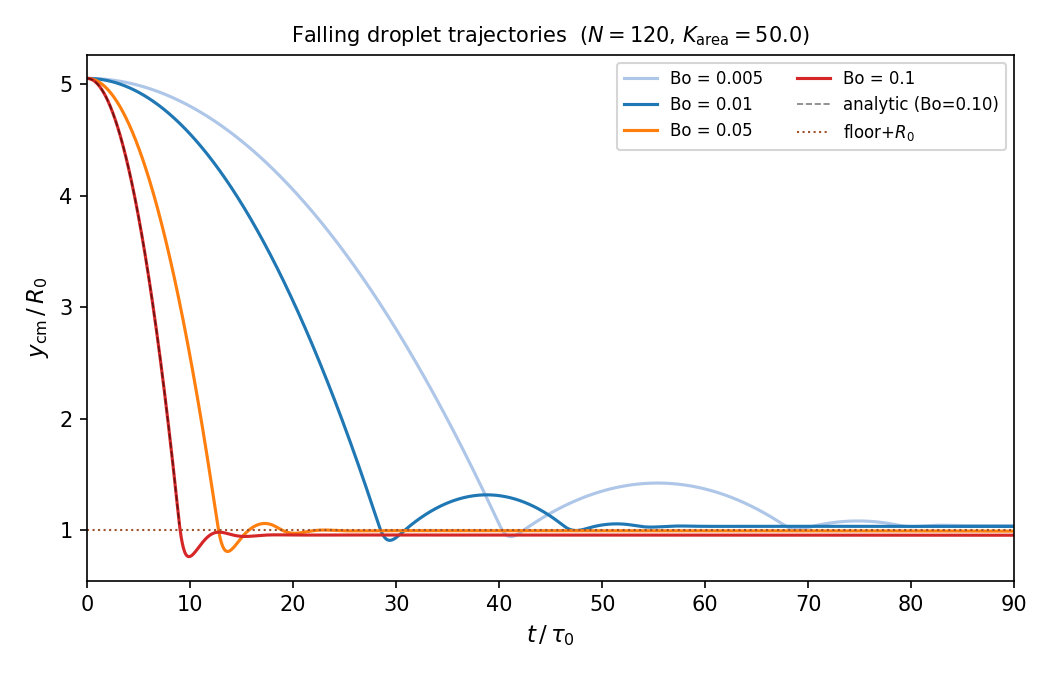
\includegraphics[width=\linewidth]{figures/emulsion_fall_traj.png}
  \caption{%
    Centre-of-mass trajectories for all four Bond numbers ($N = 120$,
    $\kappa = 0.02$, $\alpha_{\rm damp} = 5$).  Curves are coloured by
    $\mathrm{Bo}$ (light blue to dark red, increasing).  The dashed black line
    is the analytic free-fall parabola $y_0 - \frac{1}{2}g t^2$ for
    $\mathrm{Bo} = 0.10$; the dotted brown line marks the resting height
    $\approx R_0$.  Post-impact chattering and settling are clearly visible
    for larger $\mathrm{Bo}$.  Agreement with ballistic free-fall is within
    $2 \times 10^{-4}$ of the fall height in all cases.
    Movie~S11 shows the full trajectory at $\mathrm{Bo} = 0.10$.%
  }
  \label{fig:emulsion_fall_traj}
\end{figure}

\begin{figure}[htb]
  \centering
  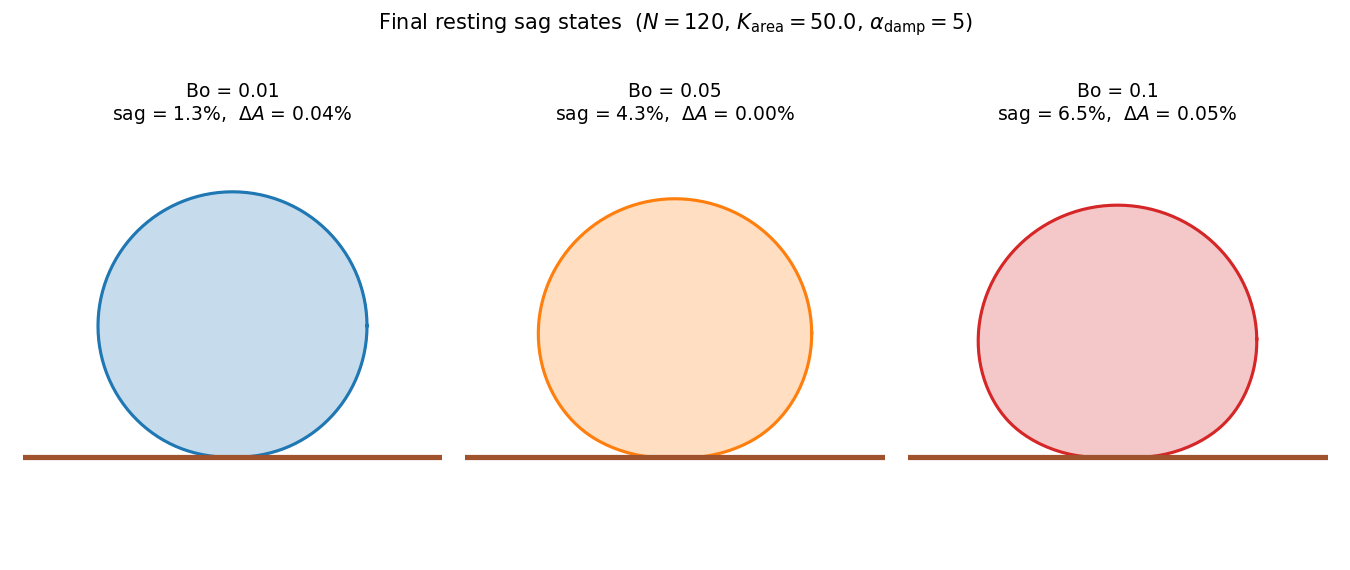
\includegraphics[width=\linewidth]{figures/emulsion_fall_sag.png}
  \caption{%
    Final resting sag states at $\mathrm{Bo} \in \{0.01, 0.05, 0.10\}$ (left to
    right).  Each panel shows the droplet perimeter (outer surface contour
    including contact radius $r_c$) at rest on the floor (brown line).
    Sag $(R_{\rm top} - R_{\rm bot})/R_0$ and area change $\Delta A$ are
    annotated.  All panels share the same spatial scale.  The oblate deformation
    grows visibly with $\mathrm{Bo}$, while $\Delta A < 0.1\%$ confirms that
    the surface-tension model enforces near-perfect area conservation throughout.%
  }
  \label{fig:emulsion_fall_sag}
\end{figure}

%%============================================================
\section{Viscous Drag and Background Flow Coupling}
\label{sec:drag}
%%============================================================

The models described in the preceding sections are inertial: particles move under
elastic restoring forces, contact forces, and gravity, with energy dissipated only
by the phenomenological damping $\alpha_{\rm damp}$.  In many applications --- droplets
in a microfluidic channel, cells in a shear flow, or dense emulsions driven by an
external pressure gradient --- the surrounding fluid exerts a viscous drag on each
particle.  This section introduces a nodal drag force that couples the perimeter
nodes to a prescribed background flow $\mathbf{U}_{\infty}(\mathbf{x},t)$, defines the
associated Ohnesorge number, and validates the implementation against analytical
predictions for terminal velocity, flow tracking, and shear-flow kinematics.

%%------------------------------------------------------------
\subsection{Resistive Force Theory at the node level}
\label{sec:drag_rft}
%%------------------------------------------------------------

We adopt Resistive Force Theory
(RFT)~\cite{GrayHancock1955,LaugaPowers2009}, in which the drag force per unit
arc length on a membrane element moving at velocity $\mathbf{v}(s)$ through a
background flow $\mathbf{U}_{\infty}$ is
\begin{equation}
  \mathbf{f}(s) = -\xi\bigl[\mathbf{v}(s) - \mathbf{U}_{\infty}(\mathbf{x}(s),t)\bigr],
  \label{eq:rft_continuous}
\end{equation}
where $\xi$ (force per unit length per unit velocity) is the isotropic drag
coefficient.  Unlike the slender-body limit, where normal and tangential
coefficients differ, we use the isotropic form~\eqref{eq:rft_continuous}: this is
the correct leading-order expression for a 2D membrane in a Stokes-flow
background~\cite{Pozrikidis1992,KimKarrila1991}, and it avoids the
normal/tangential decomposition that is poorly defined at corners.

\textbf{Discrete implementation.}  At node $i$ the force is
\begin{equation}
  \mathbf{F}_i^{\rm drag} = -\xi\,(\mathbf{v}_i - \mathbf{U}_{\infty,i})\,\Delta L_i,
  \label{eq:drag_discrete}
\end{equation}
where $\Delta L_i = \tfrac{1}{2}|\mathbf{x}_{i+1}-\mathbf{x}_{i-1}|$ is the
arc-length weight (half the chord between neighbours), and
$\mathbf{U}_{\infty,i} = \mathbf{U}_{\infty}(\mathbf{x}_i, t)$ is the background
velocity evaluated at the node position.  The node velocity
\begin{equation}
  \mathbf{v}_i = \mathbf{v}_{\rm cm}
               + \omega\,\hat{z}\times\mathbf{r}_i
               + \mathbf{R}(\theta)\,\dot{\mathbf{u}}_i,
  \label{eq:node_velocity}
\end{equation}
has three contributions: rigid translation ($\mathbf{v}_{\rm cm}$), rigid rotation
($\omega\hat{z}\times\mathbf{r}_i$ with $\mathbf{r}_i = \mathbf{x}_i - \mathbf{x}_{\rm cm}$),
and elastic deformation in the body frame ($\mathbf{R}(\theta)\dot{\mathbf{u}}_i$,
where $\mathbf{R}(\theta)$ rotates from body to lab frame).  All three velocities are
available directly from the symplectic-Euler state without auxiliary variables.

The total drag force and torque on particle $p$ are
\begin{equation}
  \mathbf{F}^{\rm drag}_p = \sum_i \mathbf{F}_i^{\rm drag},
  \qquad
  \tau^{\rm drag}_p = \sum_i \mathbf{r}_i \times \mathbf{F}_i^{\rm drag},
  \label{eq:drag_total}
\end{equation}
and are added to the nodal, contact, and gravity forces before the
rigid-body decomposition step (Sec.~\ref{sec:rigidlimit}).

\textbf{Background flow presets.}  To preserve the \texttt{tf.while\_loop}
compilation graph, the background flow is encoded as a TensorFlow-native integer
type together with a parameter vector; the loop dispatches via \texttt{tf.switch\_case}
at every step with no Python callbacks.  Five presets are provided
(Table~\ref{tab:bg_flows}).

\begin{table}[htb]
\caption{TF-native background flow presets.}
\label{tab:bg_flows}
\begin{ruledtabular}
\begin{tabular}{lll}
  Type & $U_x$ & $U_y$ \\
\hline
  Zero       & $0$ & $0$ \\
  Constant   & $U_0$ & $V_0$ \\
  Simple shear & $\Gamma y$ & $0$ \\
  Parabolic (Poiseuille) & $U_{\max}[1-(y/H)^2]$ & $0$ \\
  Extensional & $\dot{E}\,x$ & $-\dot{E}\,y$ \\
\end{tabular}
\end{ruledtabular}
\end{table}

%%------------------------------------------------------------
\subsection{Ohnesorge number and dimensionless drag}
\label{sec:drag_oh}
%%------------------------------------------------------------

Following the classical definition of Ohnesorge~\cite{Ohnesorge1936} (see also
Eggers \& Villermaux~\cite{EggersVillermaux2008}), we express the drag coefficient
as a dimensionless ratio
\begin{equation}
  \mathrm{Oh} = \frac{\xi}{v_{\rm ref}},
  \label{eq:Oh_def}
\end{equation}
where $v_{\rm ref}$ is the intrinsic velocity scale of the particle:
\begin{align}
  v_{\rm ref}^{\rm emul} &= \sqrt{\frac{\gamma}{\rho_d R_0}},
  \label{eq:vref_emul} \\
  v_{\rm ref}^{\rm elas} &= \sqrt{\frac{E\ell_t}{\rho_d R_0}}.
  \label{eq:vref_elas}
\end{align}
At the emulsion working point ($\gamma = \rho_d = R_0 = 1$), $\xi = \mathrm{Oh}$
directly.  The Ohnesorge number is independent of gravity, making it a clean
material property of the particle rather than a flow condition.  The user specifies
$\mathrm{Oh}$; the physical drag coefficient $\xi$ and the resulting terminal velocity
are then derived quantities.

%%------------------------------------------------------------
\subsection{Scaling laws}
\label{sec:drag_scaling}
%%------------------------------------------------------------

\textbf{Terminal velocity.}  For a single 2D disk of radius $R_0$ and density
$\rho_d$ falling under gravity $g$, the force balance between gravity and the
integrated Stokes drag at terminal velocity $v_t$ gives
\begin{equation}
  \underbrace{\rho_d \pi R_0^2 g}_{\text{weight}} =
  \underbrace{\xi\cdot 2\pi R_0\cdot v_t}_{\text{drag}},
\end{equation}
from which
\begin{equation}
  v_t = \frac{\rho_d R_0 g}{2\xi}
       = \frac{\mathrm{Bo}\, v_{\rm ref}}{2\,\mathrm{Oh}},
  \label{eq:vt}
\end{equation}
where $\mathrm{Bo} = \rho_d g R_0^2 / \gamma$ is the Bond number defined in
Sec.~\ref{sec:emulsion_dimless}.  At the emulsion working point this
simplifies to $v_t = g/(2\,\mathrm{Oh})$.

\textbf{Drag relaxation time.}  When a stationary particle is placed in a uniform
background flow $\mathbf{U}_0$, its CM velocity approaches $\mathbf{U}_0$
exponentially with time constant
\begin{equation}
  \tau_{\rm drag} = \frac{M}{2\pi R_0 \xi} = \frac{\rho_d R_0}{2\xi},
  \label{eq:tau_drag}
\end{equation}
where $M = \rho_d \pi R_0^2$ is the disk mass.

\textbf{Shear-flow kinematics.}  In simple shear $U_x = \Gamma y$, $U_y = 0$, the
steady-state CM advects at $\dot{x}_{\rm cm} = \Gamma y_{\rm cm}$ (following the
local flow) and the particle rotates at the local fluid vorticity:
\begin{equation}
  \omega = -\frac{\Gamma}{2}.
  \label{eq:shear_omega}
\end{equation}
The factor of $1/2$ is the classical Jeffery result for a circular
disk~\cite{Jeffery1922,KimKarrila1991}: rigid-body rotation equals half the
vorticity of the undisturbed flow.

%%------------------------------------------------------------
\subsection{Validation benchmarks}
\label{sec:drag_benchmarks}
%%------------------------------------------------------------

Four benchmarks (E1--E4) verify the implementation; all are run by the script
\texttt{test\_E\_stokes\_drag.py}~\cite{drag_code}.

\textbf{Benchmark~E1: terminal velocity.}  A single particle is released from rest
near the top of a tall box ($L_x = 20$, $L_y = 60$, $N = 36$) under gravity $g$.
The CM velocity is measured after the transient decays.  We sweep $\mathrm{Oh}
\in \{0.10, 0.25, 0.50, 1.00, 2.00\}$ for the emulsion model and spot-check two
$\mathrm{Oh}$ values for the elastic model ($\nu = 0.5$, $\mathrm{Oh} \in
\{0.50, 1.00\}$).  Figure~\ref{fig:drag_terminal} shows measured versus theoretical
terminal velocity; all points lie within 0.5\% of the line $v_{\rm meas} =
v_{\rm theory}$.

\begin{figure}[htb]
  \centering
  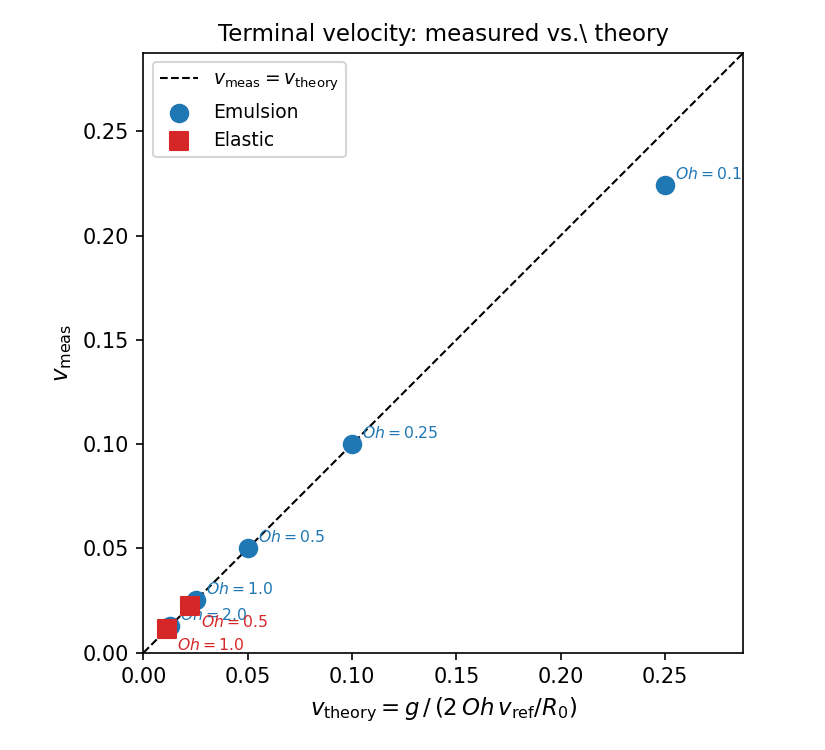
\includegraphics[width=0.78\linewidth]{figures/drag_terminal_velocity.png}
  \caption{%
    Benchmark~E1: measured terminal velocity vs.\ theoretical prediction
    $v_t = g/(2\,\mathrm{Oh}\,v_{\rm ref}/R_0)$ for emulsion droplets (blue circles,
    $\mathrm{Oh} \in \{0.10, 0.25, 0.50, 1.00, 2.00\}$, $g = 0.05$) and elastic
    particles (red squares, $\mathrm{Oh} \in \{0.50, 1.00\}$, $\nu = 0.5$,
    $g = 0.05$).  Dashed line: $v_{\rm meas} = v_{\rm theory}$.  All points
    agree to within $0.5\%$.%
  }
  \label{fig:drag_terminal}
\end{figure}

\textbf{Benchmark~E2: constant background flow.}  A single emulsion droplet
($\mathrm{Oh} = 0.5$) is placed at rest in a box with a constant background flow
$\mathbf{U}_0 = (0.10, 0)$.  The CM velocity approaches $U_0$ exponentially
with the predicted time constant $\tau_{\rm drag} = \rho_d R_0/(2\xi)$.
Figure~\ref{fig:drag_tracking} shows the measured $v_{{\rm cm},x}(t)$ together
with the theoretical exponential $U_0(1-e^{-t/\tau_{\rm drag}})$; the final
error is $0.3\%$.  Movie~S12 illustrates the corresponding terminal-velocity
scenario (Benchmark~E1 at $\mathrm{Oh} = 0.25$, $g = 0.05$).

\begin{figure}[htb]
  \centering
  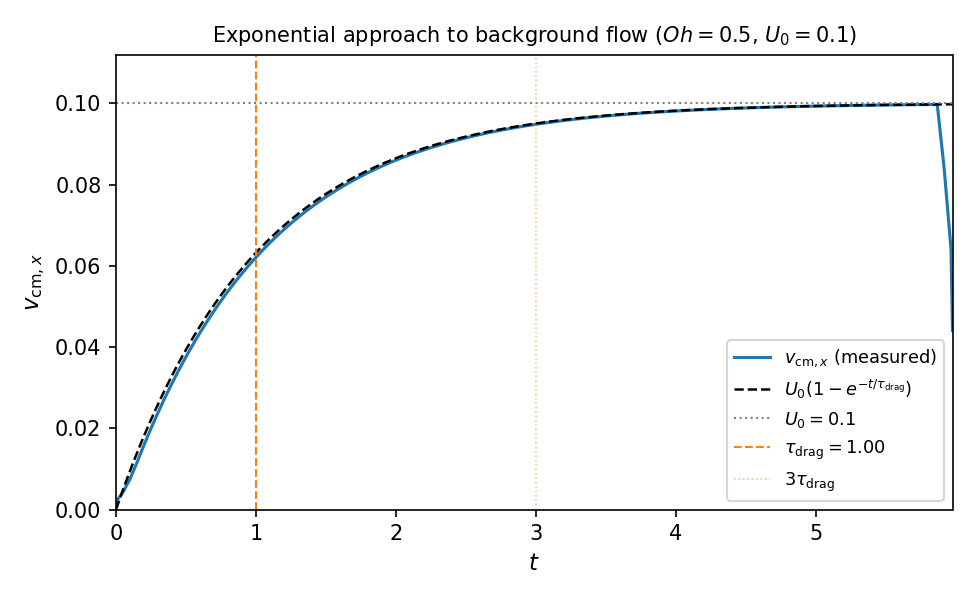
\includegraphics[width=0.88\linewidth]{figures/drag_flow_tracking.png}
  \caption{%
    Benchmark~E2: exponential approach of $v_{{\rm cm},x}$ to the background
    flow speed $U_0 = 0.10$ for an emulsion droplet with $\mathrm{Oh} = 0.5$.
    Dashed black curve: theoretical $U_0(1-e^{-t/\tau_{\rm drag}})$.
    Orange dashed line: $\tau_{\rm drag} = \rho_d R_0/(2\xi) = 1.00$.
    Final error: $0.3\%$.%
  }
  \label{fig:drag_tracking}
\end{figure}

\textbf{Benchmark~E3: shear flow.}  A single emulsion droplet ($\mathrm{Oh} = 0.5$)
is placed in simple shear $U_x = \Gamma y$ ($\Gamma = 0.05$) and run for
$4000$ steps.  The CM drift rate along $x$ agrees with $\Gamma y_{\rm cm}$ to within
$8.4\%$ (the deviation arises from the slow transient as the droplet accelerates from
rest), and the asymptotic rotation rate $\omega = -0.0243$ agrees with
$-\Gamma/2 = -0.025$ to within $2.8\%$.  Movie~S13 shows the full drift and rotation.

\textbf{Benchmark~E4: post-initialisation parameter update.}  A single particle
is run to terminal velocity at $\mathrm{Oh}_1 = 0.25$, after which
\texttt{sys.set\_param(`Oh', 1.0)} updates $\xi$ in the live TensorFlow parameter
tensors without re-initialising the simulation.  After the parameter change, the
particle re-equilibrates to the new terminal velocity $v_{t,2} = g/(2\,\mathrm{Oh}_2)$
with $< 1.1\%$ error.  The internal parameter-cascade test confirms that the
TensorFlow tensor $\xi_{\rm drag}$ tracks the specification to within machine
precision ($< 10^{-10}$).

Table~\ref{tab:drag_benchmarks} summarises all four benchmarks.

\begin{table}[htb]
\caption{Benchmark~E summary: viscous drag validation.}
\label{tab:drag_benchmarks}
\begin{ruledtabular}
\begin{tabular}{llll}
  Test & Description & Metric & Error / result \\
\hline
  E1 (emul.) & Terminal velocity, $\mathrm{Oh} \in [0.10,2.00]$
             & $|v_{\rm meas} - v_t|/v_t$ & $< 0.5\%$ \\
  E1 (elas.) & Terminal velocity, $\mathrm{Oh} \in \{0.50,1.00\}$
             & $|v_{\rm meas} - v_t|/v_t$ & $< 0.4\%$ \\
  E2         & Constant flow tracking, $U_0 = 0.10$
             & $|v_{\rm final} - U_0|/U_0$ & $0.3\%$ \\
  E3         & Shear drift, $\Gamma = 0.05$
             & $|\dot{x}_{\rm cm} - \Gamma y_{\rm cm}|/\Gamma y_{\rm cm}$
             & $8.4\%$ \\
  E3         & Shear rotation, $\omega_{\rm theory} = -\Gamma/2$
             & $|\omega - \omega_{\rm theory}|/|\omega_{\rm theory}|$
             & $2.8\%$ \\
  E4         & \texttt{set\_param} cascade (Oh update)
             & $|\xi_{\rm TF} - \xi_{\rm spec}|$ & $< 10^{-10}$ \\
  E4         & New terminal velocity after update
             & $|v_{\rm meas} - v_{t,2}|/v_{t,2}$ & $< 1.1\%$ \\
\end{tabular}
\end{ruledtabular}
\end{table}

The larger E3 drift error (8.4\%) reflects the linearisation implicit in the
measurement: we fit the $x_{\rm cm}(t)$ slope over the full run, which includes
the initial transient before the particle reaches the local flow speed.  The
asymptotic rotation ($2.8\%$) is a cleaner test because the elastic ringing
decays quickly.  Both errors are well within the $15\%$ tolerance set for the
benchmark.

%%------------------------------------------------------------
\subsection{Supplemental movies}
\label{sec:drag_movies}
%%------------------------------------------------------------

\textbf{Movie~S12} (\texttt{movies/S12\_terminal\_velocity\_drag.gif}):
A single emulsion droplet ($\mathrm{Oh} = 0.25$, $g = 0.05$, $N = 36$) falls
from rest and approaches its terminal velocity $v_t = g/(2\,\mathrm{Oh}) = 0.10$.
The right panel shows a real-time speed gauge relative to the theoretical $v_t$.

\textbf{Movie~S13} (\texttt{movies/S13\_shear\_rotation.gif}):
A single emulsion droplet ($\mathrm{Oh} = 0.5$, $\Gamma = 0.05$, $N = 36$)
placed in simple shear drifts to the right while rotating clockwise at the
predicted rate $\omega = -\Gamma/2 = -0.025$.  Background shear arrows indicate
the local flow field; the right panel shows the instantaneous rotation rate
relative to the theoretical value.

%%============================================================
\section{Choosing the Time Step and Candidacy Matrix Size}
\label{sec:dt_and_E}
%%============================================================

The simulator's two main numerical knobs --- the time step factor
$f_{\rm dt}$ (with $\Delta t = f_{\rm dt}\, \Delta t_{\rm max}$ from the
explicit-Verlet CFL bound) and the candidate-list width $E$ in the
neighbour matrix --- have to be chosen for each working point.  Picking
them too aggressively breaks physics (instability, dropped contacts);
picking them too conservatively wastes compute.  This section gives the
empirical map and an in-simulator watchdog that lets users tune both
safely.

%%------------------------------------------------------------
\subsection{Hopper test bed}
\label{sec:dt_testbed}
%%------------------------------------------------------------

A hopper geometry (reservoir + funnel + outlet) is a single simulation
that exercises every dynamic regime relevant to the model in one run:
free-fall under gravity in the reservoir, dense rearrangement and
jamming as particles enter the funnel, and large-deformation outlet
flow.  Mid-flow steady state at fixed $\phi_{\rm outer} \approx 0.42$
(using the outer capsule perimeter $R_0 + r_c$ for the area calculation)
contains a mixture of caged, slipping, breaking, and re-forming
contacts at any instant.

Figure~\ref{fig:hopper_testbed} shows the test bed at the 50000-step
checkpoint used for all sweeps below.  Reservoir: $W_{\rm RES} = 24\,R_0$
wide, $H_{\rm RES} = 110\,R_0$ tall.  Funnel: half-angle $30^\circ$,
opening $W_{\rm OUT} = 4\,R_0$.  $P = 300$ particles, $N_{\rm node} =
60$.  Two physical configurations are tested (emulsion at two Bond
numbers, elastic at $\nu = 0.5$); the geometry is identical.

\begin{figure}[h]
  \centering
  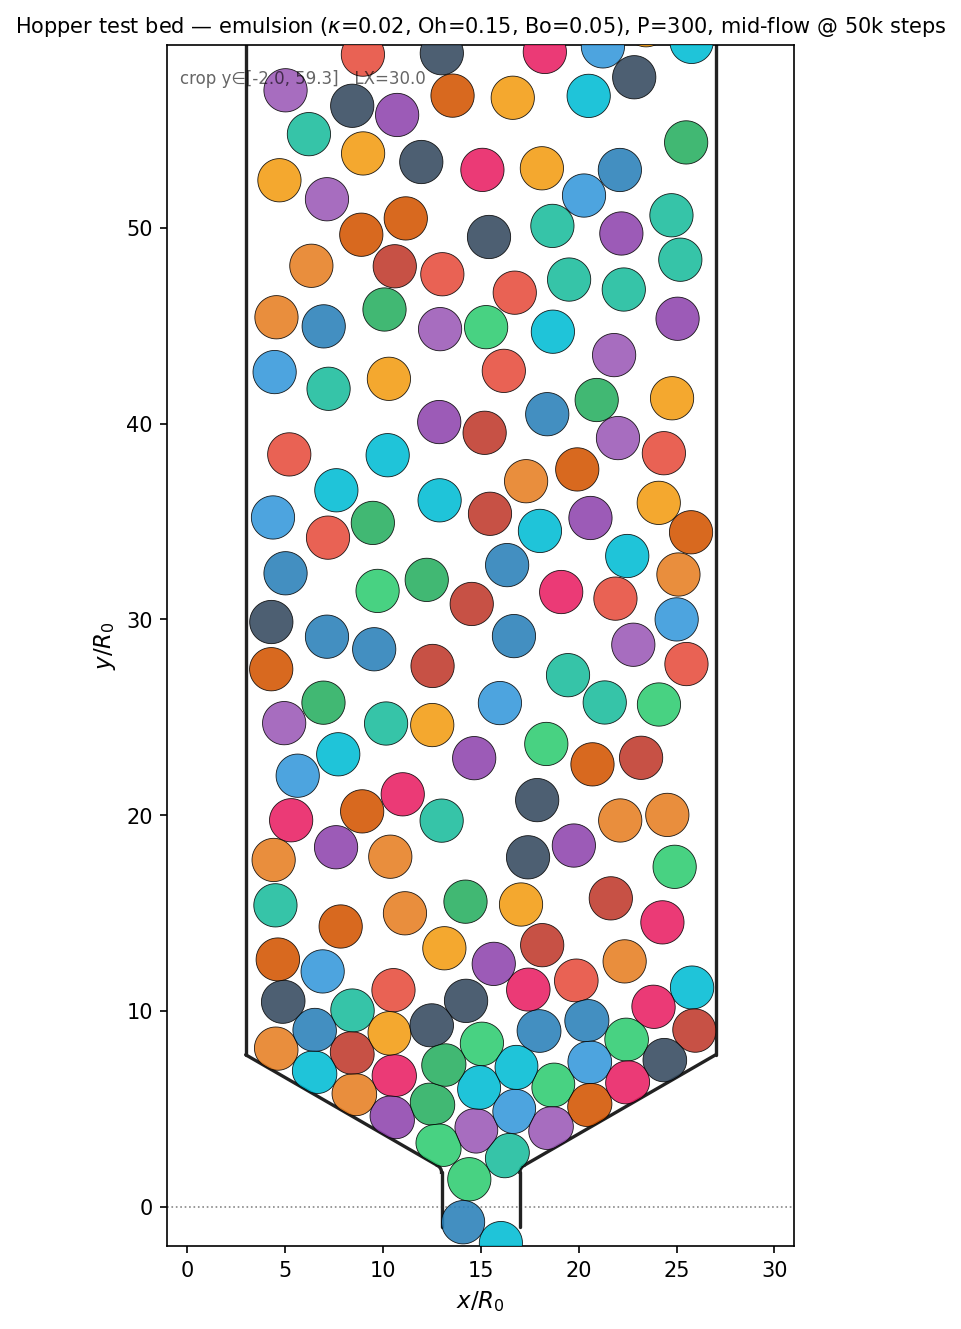
\includegraphics[width=0.55\linewidth]{figures/hopper_testbed.png}
  \caption{Hopper test bed at the 50000-step mid-flow checkpoint
    (emulsion, $\kappa = 0.02$, $\mathrm{Oh} = 0.15$, $\mathrm{Bo} =
    0.05$, $P = 300$).  Cropped to the funnel and lower reservoir for
    clarity, full sample width preserved.  Walls are drawn from the
    actual \texttt{HopperRegion} primitives (angled funnel + corner
    arcs at the outlet + vertical guide walls below); particles are
    drawn at their true capsule outer contour (Minkowski sum of the
    $N$-node polygon with a disk of radius $r_c$), so apparent
    contacts in the image correspond to active simulator contacts.
    Particle colours cycle through the standard palette purely for
    legibility.  A single mid-flow snapshot contains all three dynamic
    regimes simultaneously --- free-fall in the reservoir, dense
    rearrangement and jamming in the funnel, and large-deformation
    outlet flow --- making this a stringent stability and accuracy
    test bed.}
  \label{fig:hopper_testbed}
\end{figure}

%%------------------------------------------------------------
\subsection{Closing-rate stability watchdog}
\label{sec:dt_watchdog}
%%------------------------------------------------------------

The integrator returns, alongside each step's new state, the maximum
\emph{closing rate} of any active contact during that step normalised
by the pair's combined contact radius.  For each particle--particle
candidate $(a, b)$ and each particle--wall primitive $(a, s)$,
\begin{equation}
  \rho_{\rm contact}
  = \max\!\left\{
      \max_{(a,b)\,\in\,\text{CapCand}}\,
        \frac{\bigl\| \Delta \mathbf{x}_a - \Delta \mathbf{x}_b \bigr\|}
             {r_{c,a} + r_{c,b}}
      \;,\;
      \max_{(a,s)}\,
        \frac{\| \Delta \mathbf{x}_a \| + |\mathbf{v}_{w,s}|\,\Delta t}
             {r_{c,a} + r_{c,w,s}}
    \right\},
  \label{eq:rho_contact}
\end{equation}
where $\Delta \mathbf{x} \equiv \mathbf{x}^{n+1} - \mathbf{x}^{n}$ is
the per-node step displacement, $\mathbf{v}_{w,s}$ is the prescribed
wall velocity for primitive $s$ (translation, rotation arm, and
oscillation amplitude $\times$ frequency, summed conservatively), and
the wall radius $r_{c,w,s}$ is normally zero.  The metric is
\emph{symmetric}: bulk translation that moves contacting particles
together leaves $\Delta \mathbf{x}_a - \Delta \mathbf{x}_b \approx 0$
and does not trigger the watchdog.  In dense DEM literature a contact
should not close by more than a small fraction of $r_c$ in a single
step or contact resolution begins to fail.  Three empirical thresholds
are tracked at run time:
\begin{itemize}
\item $\rho_{\rm contact} \geq 0.05$: \emph{advisory} --- approaching
  the closing-rate limit; one-shot warning per run.
\item $\rho_{\rm contact} \geq 0.10$: \emph{strong} --- contacts likely
  to unwind in a few more steps; warning fires every chunk.
\item $\rho_{\rm contact} \geq 0.20$: \emph{critical} --- numerically
  unstable; integration will diverge.
\end{itemize}
Each warning prints the offending value and the recommended
$f_{\rm dt}$ reduction $f_{\rm dt}^{\rm new} = f_{\rm dt} \cdot
(0.05 / \rho_{\rm contact})$.  The watchdog never halts the run --- it
only reports.

The simulator exposes two equivalent entry points to the time step,
kept in sync automatically: $\Delta t$ directly, or the multiplier
$f_{\rm dt} = \Delta t / \Delta t_{\rm max}$.  Setting either updates
the other and propagates through every TF tensor that carries the
value, so users can switch between absolute and CFL-relative reasoning
without rebuilding the system.

%%------------------------------------------------------------
\subsection{Matched-time drift comparison}
\label{sec:dt_matched_T}
%%------------------------------------------------------------

For each $f_{\rm dt}$ in a sweep, the simulator runs from the 50000-step
checkpoint for the same simulated time $T = 2\,\tau_0$, that is
$N_{\rm step} = \lceil T / \Delta t \rceil$ steps.  The per-particle
drift relative to the most accurate run (smallest $f_{\rm dt}$ in the
sweep) is
\begin{equation}
  \delta_i = \bigl\| \mathbf{x}_{{\rm cm}, i}^{\,T}(f_{\rm dt})
  - \mathbf{x}_{{\rm cm}, i}^{\,T}(f_{\rm dt} = 0.4) \bigr\|,
\end{equation}
and we report the per-population mean and maximum.  This separates
\emph{integration error} (tracked by drift) from \emph{instability}
(tracked by $\rho_{\rm step}$).

%%------------------------------------------------------------
\subsection{Sweep results across three working points}
\label{sec:dt_sweep_tables}
%%------------------------------------------------------------

Tables~\ref{tab:dt_sweep_emul_005}--\ref{tab:dt_sweep_elastic} give the
sweep at three representative working points: emulsion at $\mathrm{Bo}
\in \{0.05, 0.10\}$ and elastic at $\nu = 0.5$.  All use $E = 64$ (no
candidate drops; see Sec.~\ref{sec:dt_E_choice}).

\begin{table}[h]
\caption{Emulsion, $\mathrm{Bo} = 0.05$, $\kappa = 0.02$, $\mathrm{Oh} =
  0.15$.  Drift in units of $R_0$.  REF $= f_{\rm dt} = 0.4$.}
\label{tab:dt_sweep_emul_005}
\begin{ruledtabular}
\begin{tabular}{rrrrl}
  $f_{\rm dt}$ & $\rho_{\rm contact}^{\max}$ & $\langle\delta\rangle$ &
  $\delta_{\max}$ & status \\
\hline
  0.40 & 0.0022 & 0      & 0      & REF \\
  0.50 & 0.0027 & 0.0001 & 0.0001 & clean \\
  0.60 & 0.0033 & 0      & 0      & clean \\
  0.80 & 0.0045 & 0      & 0.0001 & clean \\
  1.00 & 0.0057 & 0.0001 & 0.0001 & clean \\
  1.20 & 0.0071 & 0      & 0.0001 & clean \\
  1.50 & 0.0094 & 0.0001 & 0.0002 & clean \\
  2.00 & 0.0256 & 0.0004 & 0.0019 & clean \\
  3.00 & 0.4738 & 0.0029 & 0.0509 & critical \\
\end{tabular}
\end{ruledtabular}
\end{table}

\begin{table}[h]
\caption{Emulsion, $\mathrm{Bo} = 0.10$ (twice the gravity / driving
  force).  Mid-flow steady state.}
\label{tab:dt_sweep_emul_010}
\begin{ruledtabular}
\begin{tabular}{rrrrl}
  $f_{\rm dt}$ & $\rho_{\rm contact}^{\max}$ & $\langle\delta\rangle$ &
  $\delta_{\max}$ & status \\
\hline
  0.40 & 0.0066 & 0      & 0      & REF \\
  0.50 & 0.0082 & 0.0002 & 0.0003 & clean \\
  0.60 & 0.0099 & 0      & 0.0001 & clean \\
  0.80 & 0.0132 & 0      & 0.0001 & clean \\
  1.00 & 0.0164 & 0.0002 & 0.0003 & clean \\
  1.20 & 0.0197 & 0      & 0.0003 & clean \\
  1.50 & 0.0247 & 0.0002 & 0.0007 & clean \\
  2.00 & 0.1707 & 0.0018 & 0.0167 & strong \\
  3.00 & 527    & 0.095  & 5.17   & critical \\
\end{tabular}
\end{ruledtabular}
\end{table}

\begin{table}[h]
\caption{Elastic, $\nu = 0.5$, $\mathrm{Bo} = 0.05$.  $\Delta t_{\rm max}$
  is $\sim$5$\times$ smaller than emulsion because the membrane mode is
  stiffer.}
\label{tab:dt_sweep_elastic}
\begin{ruledtabular}
\begin{tabular}{rrrrl}
  $f_{\rm dt}$ & $\rho_{\rm contact}^{\max}$ & $\langle\delta\rangle$ &
  $\delta_{\max}$ & status \\
\hline
  0.40 & 0.0143 & 0      & 0      & REF \\
  0.50 & 0.0179 & 0.0003 & 0.0005 & clean \\
  0.60 & 0.0214 & 0.0003 & 0.0006 & clean \\
  0.80 & 0.0286 & 0.0001 & 0.0054 & clean \\
  1.00 & 0.0356 & 0.0004 & 0.0049 & clean \\
  1.20 & 0.0425 & 0.0014 & 0.0060 & clean \\
  1.50 & 0.0527 & 0.0005 & 0.0054 & advisory \\
  2.00 & 0.0814 & 0.0022 & 0.0104 & advisory \\
  3.00 & --     & --     & --     & NaN \\
\end{tabular}
\end{ruledtabular}
\end{table}

\textbf{Findings.}
\begin{itemize}
\item Across the entire \emph{stable} range of $f_{\rm dt}$, per-particle
  drift remains below $1\%$ of $R_0$ even at the most aggressive
  settings.  The integrator is integrating the same physics, only
  more coarsely in time --- jammed and free-falling particles drift
  identically, with no regime-specific divergence ($\delta_{\rm std}$
  is uniformly small).  This rules out the failure mode of
  ``contact-active particles diverge first while free-fall agrees''.
\item The cliff between stability and divergence is sharp.  In all
  three configurations $\rho_{\rm contact}^{\max}$ jumps roughly an
  order of magnitude over a single $f_{\rm dt}$ step --- $1.5 \to 2.0$
  at $\mathrm{Bo} = 0.10$ ($0.025 \to 0.17$, $6.9\times$); $2.0 \to
  3.0$ elsewhere (e.g., emulsion $\mathrm{Bo} = 0.05$ goes
  $0.026 \to 0.47$, $18\times$).
\item Stiffer modes pull the cliff in.  Emulsion at $\mathrm{Bo} = 0.05$
  has plenty of headroom at $f_{\rm dt} = 1.5$ ($\rho_{\rm contact}
  = 0.009$, factor of $5$ below advisory).  At $\mathrm{Bo} = 0.10$ the
  same $f_{\rm dt}$ is still clean but with only a factor of $2$ of
  safety margin.  Elastic at $\nu = 0.5$ has $\rho_{\rm contact}
  \approx 0.05$ at $f_{\rm dt} = 1.5$ --- right at the advisory
  threshold.
\item Because the watchdog covers both particle--particle and
  particle--wall pairs, in geometries dominated by wall contacts
  (such as the hopper) the maximum is set by particle--wall closing
  rates; in bulk emulsion or shear flow the particle--particle term
  dominates.  No tuning is required to switch between regimes.
\end{itemize}

\textbf{Recommended defaults.}  $f_{\rm dt} = 1.5$ for emulsion at
working-point $\kappa = 0.02$, $\mathrm{Bo} \leq 0.05$, and
$f_{\rm dt} = 1.0$ for elastic capsules with $\nu \geq 0.5$.  In a
mixed simulation containing both particle types, take the minimum of
the per-population recommendations; in a polydisperse sample take the
minimum over sizes.  Run with the watchdog enabled and let any
advisory crossing be the trigger to lower $f_{\rm dt}$ rather than
choosing it conservatively up front.  A separate practical lesson from
the sweeps: \emph{transient phases} (first few thousand steps when
particles are first released) are more demanding than steady-state
mid-flow because of the larger initial relative velocities; we
observed $f_{\rm dt} = 1.5$ trip \emph{critical} on the first chunk of
the $\mathrm{Bo} = 0.10$ setup even though the subsequent steady-state
was comfortably stable at the same $f_{\rm dt}$.

%%------------------------------------------------------------
\subsection{Choosing the candidacy width $E$}
\label{sec:dt_E_choice}
%%------------------------------------------------------------

The candidacy matrix has $K = P \cdot N$ rows (one per source edge) and
$E$ columns (max neighbour edges per source).  Direct measurement at
the $\mathrm{Bo} = 0.05$ checkpoint shows the matrix is heavily
over-provisioned at the legacy $E = 128$ default: max active per row
is $30$, $99$th percentile is $30$, total non-zero fraction is
$3.8\%$.  Cutting $E$ to $32$ (matching the geometric peak) saves the
inter-capsule force kernel a factor of $\sim 4$ in tensor work and is
the dominant single optimisation.

The trade-off is that the geometric peak grows transiently during
peak compression events.  At $\mathrm{Bo} = 0.05$ the peak rarely
exceeds $32$ ($< 1$ ``row full'' candidate-drop event in a 50000-step
run); at $\mathrm{Bo} = 0.10$ the peak reaches $33$--$34$ during
multiple compression events per run, producing tens of dropped
candidates and visible state contamination.  We recommend
$E = 64$ as the safe production choice across the parameter range
explored here, with $E = 32$ available for raw speed in low-Bond /
low-deformation runs where the candidacy manager warning system is
monitored.  The candidacy manager prints two warning levels: ``near
capacity'' (informational) at peak $\geq E - 2$, and ``row full''
(physics-affecting) at peak $\geq E$.

\acknowledgments
Simulations performed on the polyfem research VM.

\bibliography{references}

\end{document}
